\documentclass[a4paper,11pt]{article}
\usepackage[utf8]{inputenc}
\usepackage{graphicx}
\usepackage{amsmath}
\usepackage{titling}
%\usepackage[sorting=none,style=numeric-comp]{biblatex}
%\addbibresource{mybib.bib}
\usepackage{float}
\usepackage[top=2.5cm, bottom=2.5cm, left=2.5cm, right=2.5cm]{geometry}
%\usepackage[backend=bibtex,style=numeric,sorting=none]{biblatex}
\usepackage[style=nature, language=auto, autolang=other, backend=bibtex, sorting=none]{biblatex}
\addbibresource{lib.bib}
\usepackage{eurosym}
\usepackage{appendix}
\usepackage{xcolor}
\usepackage{array}
\usepackage{makecell}
\usepackage{caption}
\usepackage[most]{tcolorbox}
\usepackage{url}

%\usepackage{afterpage}

%\usepackage{titlesec}
%\flushbottom

\definecolor{darkblue}{rgb}{0.0, 0.0, 0.55}
\definecolor{coolblack}{rgb}{0.0, 0.18, 0.39}
\definecolor{linkcolor}{rgb}{0,0,0.65} %hyperlink
\definecolor{royalblue(web)}{rgb}{0.25, 0.41, 0.88}
\definecolor{bluegray}{rgb}{0.4, 0.6, 0.8}
\definecolor{royalblue(traditional)}{rgb}{0.0, 0.14, 0.4}
\definecolor{SlateGray1}{rgb}{198, 226, 255}
\definecolor{Snow3}{RGB}{205, 201, 201}

\definecolor{boxcolor}{RGB}{238, 233, 233}

\usepackage[colorlinks=true, linkcolor=black, urlcolor=royalblue(traditional), citecolor=black]{hyperref}

\captionsetup[figure]{name=Fig.}

\title{\textbf{Stereotypes and fraud: can common knowledge identify fragile subjects?}}
\author{Carlo Arpini 918543 - Emmanuele Lotano 918608 - Chiara Mariani 918354}
\date{}

\begin{document}

\sloppy

\begin{center}
    \small \
    Course of Data Science Lab - Professor M. Fattore and S. Gerli - Academic year 2023/2024  \\
    \vspace{0.5cm}
    \huge
    \thetitle \\
    \vspace{0.5cm}
    \large
    \theauthor \\
    \vspace{0.4cm}
    \small \textit{Università degli Studi di Milano-Bicocca, CdLM Data Science}
    
\end{center}

\vspace{0.8cm}
\hrule
\vspace{0.8cm}

\begin{abstract}
\begin{tcolorbox}[
    width=14cm,
    height=3.72cm,
    colback=boxcolor,
    colframe=white,
    arc=5pt,
    outer arc=5pt,
    left=0pt,
    right=0pt,
    top=0pt,
    bottom=0pt,
    boxsep=5pt
]

  Within the digital age, financial frauds have found new fertile terrain thanks to newly birthed products and ease of use of instruments that move capital. Our research tries to identify links between common financial attributes and one's fragility and vulnerability to financial frauds through a 2017 survey proposed by Bank of Italy to which we applied Machine Learning methods. The results highlight some common factors that are within the domain of public knowledge but also a systematic aspect to frauds that applies to everyone and other aspects that encompass the Italian landscape, such as a low financial knowledge and a debt averse society. 

%\textcolor{darkblue}{\rule{1pt}}
\end{tcolorbox}
\end{abstract}


\tableofcontents

\newpage
\section{Introduction}
\subsection{Context of our analysis}
In the digital context in which Italian citizens live every day, information technology has transformed each of our lives into an existence rooted in an online environment. This has brought with it not only benefits, such as the speed of information propagation and the possibility of immediate global comparison, but also numerous harms, including a pathological dependence on digital and an impoverishment of human  relationships. A further negative aspect of digital society that has been on the rise in recent years is the issue of online financial fraud. The advent of online transactions, the emergence of e-banking and the digitalisation of international economies have increased the risk of being a victim of online fraud, affecting a significant portion of the population, regardless of age, gender or social background.\\

In Italy, cyber frauds are considered a phenomenon that constantly threatens customers and banks. In this regard, \href{https://bari.corriere.it/notizie/cronaca/24_settembre_01/conti-correnti-svuotati-con-un-clic-allarme-in-puglia-e-la-quinta-regione-in-italia-in-tanti-si-ritrovano-indebitati-66eb1381-4012-41ef-81d3-ec118796fxlk.shtml?appunica=true&app_v2=true}{Corriere del Mezzogiorno} \cite{CdM} specified that, based on data from the CRIF Observatory Report, there has been an increase in both the average amount of frauds and a change in criminal strategies. In particular, the regions most affected were Lombardy with 13.8\% of total assets stolen with frauds, Sicily with 13.2\%, Campania  with 12.7\%, Lazio and Puglia trailing close just under 10\% with 9.3\% and 8.9\% respectively. These high percentages highlight not only the ability of scammers to manipulate victims, but also the vulnerability of a good portion of the Italian population to such threats. 

%Frauds, like other criminal phenomena, have always existed; however, in an increasingly digital-dependent world, they have become a daily phenomenon. This suggests that online security and fraud prevention should not be underestimated.

\href{https://www.consob.it/web/investor-education/truffe}{CONSOB} \cite{Consob} emphasizes that online frauds pose a threat to financial stability and consumer confidence, as savings are a valuable asset that should not be evaporated in the hands of scammers. Therefore, it is necessary to take preventive measures, such as promoting greater awareness and financial education of citizens.\\

Using a \href{https://www.bancaditalia.it/statistiche/tematiche/indagini-famiglie-imprese/alfabetizzazione/Data-description.pdf?language_id=1}{questionnaire} designed by the Bank of Italy \cite{BdI} in 2017 and completed by approximately 2,500 individuals, we attempt to discern which factors determine whether or not an individual can be considered susceptible to exploitation. It will be of interest to evaluate whether the findings align with the collective imagination or deviate from conventional wisdom due to cognitive biases to guide any regulatory standpoint.

\subsection{Idea and aim of our analysis}

In the context of an environment where online frauds are a persistent and growing concern, it is crucial to identify any pattern that might be linked to being victims of a financial fraud, to act upon them. This is the central question that we address in our analysis. 

The aforementioned \href{https://www.bancaditalia.it/statistiche/tematiche/indagini-famiglie-imprese/alfabetizzazione/Data-description.pdf?language_id=1}{questionnaire} includes questions of a socio-demographic nature, such as geographic area of origin, educational qualification or employment status. It also includes questions related to financial knowledge, such as the definition of simple and compound interest or inflation. Additionally, it encompasses questions related to each individual's financial behavior, touching on topics such as savings, long-term goals or the purchase of financial instruments. \\

As a preliminary step, we identified the question in the questionnaire that pertains to whether an individual has ever been the victim of a fraud. 
Once the preliminary steps had been completed, enabling the dataset to be processed in a suitable manner, an attempt was made to consolidate the various questions into eight subcategories, thus facilitating interpretation. Three different algorithms (Random Forest, Logistic Regression and Multi Layer Perceptron) were applied to try and classify fraud victims based on the Matthews Correlation Coefficient \cite{BioData}, \cite{BMC} on both the full dataset and the dataset implemented with feature engineering. Subsequently, undersampling techniques and class weights were employed to address some inherent problems in the data distribution.
As there was a small but acceptable reduction in predictive capacity, the dataset obtained through feature engineering was selected for the final analysis given it had sufficient results but great explainability. The most significant features, as determined by Gini entropy decrease and Permutation Importance, and the relationship between each and the target variable can be investigated through Partial Dependences of each feature. These methods enabled us to forge a path in interpreting stereotypical ideas and values in the personal financial space, but ultimately demonstrated the capillary presence of frauds for all classes of victims. \\

Ultimately, we also sought to construct six prototypical profiles of individuals who might have responded to our survey based on common knowledge and common ideas to assess the likelihood of them being defrauded and to gain insights on if the stereotypes hold true or not under our analysis and what can be gained from a regulatory ``prevention - based" approach standpoint.

\section{Dataset Description}
The dataset is essentially comprised of 2376 replies by 106 columns, which can be seen in the Appendix \ref{sec:appendix}. We have such a high number of columns as multiple choice questions are represented by binary columns, which have values of ones when the choice is selected and zeros otherwise; this results in a number of columns that is almost three times that of the questions highlighted in the Appendix \ref{sec:appendix}. Because of this, any analysis done on the dataset as is is essentially uninterpretable, and we are forced to first try and clean/reduce our dataset to enhance interpretability of even the most basic analysis.

Moreover, we do not have a direct target variable but rather we have three questions that can be used to infer values of the target variable; this also calls for more data handling.
\subsection{Main pain points}
There are also some other pain points to be highlighted. First things first, not all questions were asked to participants. As an example, question \textit{``qd12"} triggers only whenever the participant replies a specific reply to question \textit{``qd11"}. As a result we have also to deal with a lot of NaN values, with the upside that they are easily interpretable; note that this is not the only example of this phenomenon in the dataset. 

At last, there are also pain points which will be present until the end by definition and will not be solvable: as an example, there is no interpretation for the \textit{``pesofitc"} column, nor we have any way of telling if a participant is truthful or not in its replies, and we may have inconsistency, which will be almost impossible to detect unless in reading and reinterpreting all the data points. Some information from the original research as such will either not be accessible and some level of uncertainty will systematically be present in the analysis.
\section{Data cleaning}
The data cleaning section will focus on handling of NaN values and a light feature reduction that will not result in losing any information that is to be considered relevant. This is after, most importantly, we recreate our target variable: a binary class called \textit{``defrauded"} that will tell us if the person has been a fraud victim or not. 
\subsection{Target variable creation}
Our dataset in itself, as mentioned in the dataset description section, does not contain a direct question that we can use to check whether a person was a fraud victim. We have to infer this possibility from three binary questions that were present, which are \textit{``qprod4\_1"}, \textit{``qprod4\_2"} and \textit{``qprod4\_3"}. 
The main line of reasoning to get the value of our target variable is the following: \textit{``qprod4\_2"} and \textit{``qprod4\_3"} refer to cases where it is undeniable the respondent has been defrauded. If the reply was a solid ``yes" to either, our target variable should be a one; in fact, \textit{``qprod4\_2"} refers to having private financial information stolen trough fraudulent phone calls and \textit{``qprod4\_3"} instead refers to respondent money being used to pay for goods without authorisation. Instead, \textit{``qprod4\_1"} is less clear: if say a person accepts investment advice on some worthless financial product from one of its relatives, it could be that they were in good faith and they too lost money; in a sense they were the fraud victim while the respondent was ``collateral damage". 

To approach this problem thus this insight might not be enough. In fact, when we consider that the possible replies for all three questions were ``yes", ``no" and ``I prefer not to answer/I don't understand/I don't know", we see we have too many options; but considering that all three options that are not the classic ``yes" or ``no" give zero value to our analysis we can group them in a general ``no information" of some sort. This way, we have $3^3$ combinations of possible cases in which we subdivide our space of answer: ``yes", ``no" and ``no information". Within this space, the reasoning that ``if we replied yes to either second or third question then the target variable is 1", already covers 15 cases; then, we have those who were surely not victims having replied 3 times ``no" as another covered possibility. 

We can furthermore notice that in 4 left possibilities the respondent replied ``yes" to the first question and either ``no" or ``no info" to the other two; in those cases we can check the \textit{``qprod3\_8"}, \textit{``qprod3\_9"} and \textit{``qprod3\_10"} questions: if the respondent replied ``yes" to either of the three we can consider that whoever suggested any financial product that was later worthless was someone that had the respondent's best interest in mind and as such he was not defrauded. Else, he was; and so we are left with 7 cases where it is unclear. 

Of those cases, we decided to flag as not fraud victims those where the replies where mostly ``no" (``no" for two questions, ``no info" for just one) and to instead delete all those rows where we essentially have not enough information because the majority of replies were neither ``yes" nor ``no". This drastic decision leads to loss of 110 data points that for our analysis can't be utilised, but gives us a completely partitioned space of data points where each data point is mapped accordingly to what said before to either 1 or 0.


\subsection{Feature reduction}
At this point we can proceed and delete some useless columns, as well as those columns we just used to create the new target variable. The other columns that brought no value and were deleted were: 
\begin{itemize}
    \item \textit{ID}: this column is essentially useless 
    \item \textit{PESOFITC}: this column too is useless since we have no knowledge of how it was assigned nor what it means
    \item \textit{SM}: this column give us no useful information
    \item \textit{qd5b}: the number of household members should not be correlated with our target variable whatsoever, and hence removing it we actually remove the possibility of introducing biases
    \item \textit{qd12}: same explanation as \textit{qd5b}
    \item \textit{qf3\_99}: this is a single column of a multiple choice answer and it is eliminated because it is redundant, in fact the column ``no answer" to multiple choice question is the same as all zeros for the other options from an absence of information standpoint
    \item \textit{qf9\_99}: same reasoning as \textit{qf3\_99}
    \item \textit{qprod1c\_99}: same reasoning as \textit{qf3\_99}
    \item \textit{qprod3\_99:} same as
    \textit{qf3\_99}
    \item \textit{qf12\_97} and \textit{qf12\_99}: same as \textit{qf3\_99}
    \item \textit{qprod1\_d}: once again this is somewhat redundant as our target variable shouldn't be affected by when a financial product was bought
\end{itemize}
After this feature reduction we are left with 92 columns.
\subsection{Data discretisation}
Another thing we can do is discretise some of the data to lower even further the number of columns and/or the width of the space of data points. As an example, it makes sense to discretise age in age ranges for both explainability and to lower the width of the space of data points. Values affected by this are:
\begin{itemize}
    \item \textit{AREA5}: discretisation groups values in North/center and South + islands
    \item \textit{qd7}: this is exactly the age ranges creation, following standard 10 year long ranges
    \item \textit{qd9}: here we are grouping education in highest \textit{completed} education
    \item \textit{qf4}: discretisation here maps answers of ``I don't know" and ``I don't have a personal income" together, because they both represent absence of data
    \item \textit{qf8}: same as \textit{qf4}
    \item \textit{qf10\_i} $\forall i$: same as \textit{qf4}
    \item \textit{qk1}: same as \textit{qf4}
    \item \textit{qf13}: same as \textit{qf4}; here we also group the first two options together
    \item \textit{qf9\_i} $\forall i$: here we group together some multiple choices; we group together \textit{qf9\_2} with \textit{qf9\_3}, \textit{qf9\_7} with \textit{qf9\_8}, \textit{qf9\_1} with \textit{qf9\_9}. This allows us to reduce further the number of columns while preserving data for two columns that were very similar as couples
    \item \textit{qprod3\_i} $\forall i$: in similar fashion as \textit{qf9\_i}, we grouped \textit{qprod3\_1} with \textit{qprod3\_16}, \textit{qprod3\_13} with \textit{qprod3\_15}, \textit{qprod3\_3} with \textit{qprod3\_6} and \textit{qprod3\_5} with \textit{qprod3\_7}, \textit{qprod3\_12} and \textit{qprod3\_14}
    \item \textit{qf12\_i} $\forall i$: here in similar fashion as \textit{qf9\_i} we aggregate \textit{qf12\_1\_c} with \textit{qf12\_3\_g} and \textit{qf12\_5\_m} with \textit{qf12\_4\_k}, \textit{qf12\_5\_o} and \textit{qf12\_6\_p}
    \item \textit{qk3} to \textit{qk7} series questions: these questions are related to financial knowledge and as such they can be viewed as a three-class correct/incorrect/blank answer; hence the discretisation criteria is exactly that
\end{itemize}
\subsection{Missing values handling}
One more manipulation that we must do is handle missing data in our dataset. This refers specifically to columns generated by questions \textit{``qf12\_i"} series, \textit{``qprod2"} and \textit{``qprod3\_i"} series, which are only asked to the respondent when he replies in a specific manner to earlier questions. This time the handling is really simple: basically whenever we see a NaN we substitute it with whatever value in that question is associated with the absence of a reply or information (usually -99). Notice how once again this has basically no impact on the data itself and is consistent and coherent.
Now, after all this work, as is the dataset is comprised of 2266 rows of data by 79 columns.
\section{Feature engineering}
Now, while our dataset is technically complete and without missing data, it still is far from easy to interpret, even despite the light aggregation on practically identical columns. We will utilise the dataset as is to train a model, but we would also like to be able to interpret the model more easily, and that can be done through feature engineering. 

More specifically the idea is the following: we want to exploit common financial clichés to check whether they can actually hold information and whether the ``fraudability" of each participant can be measured through naïve features with which most people would judge one's financial situation. This way, if machine learning models trained on those feature have similar results as those trained on the full dataset we will not have loss of information or predictive power, while having a great explainability and of easy interpretation, linked to common thought; if this is not the case, we will be anyway able to tell if that's because those naïve features are not sophisticated enough or if it's just that frauds occur at any level without any correlation to new engineered variables; effectively, we'll be able to gain knowledge and interpretability either way and in any case the result would provide guidance to any regulatory authority interested in protecting citizens. 

To transform existing features in new ones we decided to use a quasi linear combination of variables, which is described by the matrix \ref{sec:coeffweights}; the combination is almost a linear combination but sometimes we decided to either transform variables such that they were centered around zero or enhance their negative effect if they were binary. This means for example that all questions with ranges 1 to 5 (\textit{``qf10\_i"} series, \textit{``qk1"}) were rescaled with a $\Bar{x}-x_i$ transformation, and then that value was used in the linear transformation, or another example of this is the fact that for some features some instances of \textit{``qf12\_i"} or \textit{``qf9\_i"} were grouped such that even if only one was flagged as a ``yes" then the reply on the others didn't matter. 
The transformation because of this details isn't entirely linear aside for some features (as an example for ``\textit{financial knowledge}"). \\

The new features are:

\begin{itemize}

\item{\textit{\textbf{Financial knowledge}}}

The feature incorporates the survey questions that estimate respondents' financial knowledge. Specifically, these questions test financial knowledge through targeted mathematical/financial questions: respondents can enter an exact value from the keyboard or choose one of the possible answers from those reported.
The minimum theoretical possible value corresponds to -7 and the maximum theoretical possible value corresponds to 7; this range of possible results for this feature was obtained by calculating the worst and best case of the transformation. 
Note that this score has nothing to do with perceived financial knowledge, which will be defined afterwards, at least in principle

\item{\textit{\textbf{Indebtment}}}

The debtor variable shows whether the respondent of the survey leans towards debt or is debt averse. High values correspond to a tendency towards debt, while low values correspond to a debt averse person. 
The features that are included in this variable are related to different aspects of the financial situation of each respondent such as missing payments, worrying about normal living expenses or signing up for unsecured loan. 
To better understand the variable we are dealing with, we compute the lowest value in the dataset, which corresponds to -5.5, and highest value which is equal to 9.0. More precisely, we can draw our own conclusions using the theoretical minimum and maximum. The range for this feature is from -5.5 to 10.5, calculated considering the highest possible case and the lowest one of the transformation. The discrepancy between theoretical maximum and our dataset's maximum score already suggests a general debt-aversion.

\item{\textit{\textbf{Perceived financial knowledge}}}

The perceived financial knowledge tells us how much the respondent felt confident in its financial knowledge: the higher, the higher the perceived knowledge. The lowest value and the highest one within the dataset are equal to -5.25 and 6.0, which are very closed to the theoretical values of the variable that are -6.0 and 6.5. The variable is computed with questions such as \textit{``qk1"}.

\item{\textit{\textbf{Saving attitude}}}

The saving attitude variable tells how much the respondent is a saver or someone who tends to spend: the higher, the more the respondent saves. More in depth, this feature takes into account all those aspects of real life where a person is willing to spend or save money, through questions on both the actual savings and the person put in hypothetical scenarios. The lowest and highest value calculated within the dataset are equal to -6.25 and 10.85. In this case, the range of values is quite wide, which is confirmed by the theoretical minimum and maximum values of -7.75 and 15.85.

\item{\textit{\textbf{Planning attitude}}}

The planning attitude feature highlights how much the respondent plans his future or not: the higher, the more the respondent usually is able to plan for a distant (or not) future, financially speaking. Tendency to live for today and letting tomorrow take care of itself or setting long term financial goals are only two examples of what is included as planner attitude. In this cases, the lowest value within the dataset is equal to the theoretical minimum which corresponds to -8.0, while the highest value is 10.75 and the theoretical maximum is 11.75.

\item{\textit{\textbf{Financial products experience}}}

The financial products experience feature wants to measure respondents' knowledge and experience of various financial products (such as bonds, stocks, shares, mutual funds). Specifically, the questions tried to test direct financial experience.
The lowest value obtained among the respondents corresponds to -0.5, while the highest was observed to be 8.5; finally, the range of possible results for this feature was obtained by calculating the maximum and minimum of the transformation and yielded a value of -0.5 for the minimum and and the 10.6 for the maximum.

\item{\textit{\textbf{Digitalisation}}}

The digitalisation feature incorporates a series of questions designed to better understand the relationship between respondents and technology.
In particular, these questions assess the use of technological or analog products (such as cash) within the domain of financial economics.
It was observed that the lowest value obtained among the respondents was -2.2, while the highest was 1.0, while the range of possible results for this feature was obtained by calculating the maximum and minimum of the transformation: the minimum theoretical value is -3.0 and the maximum theoretical possible value is 1.0.

\item{\textit{\textbf{Independent financial approach}}}

The independent financial approach variable tells how much the respondent has a tendency in being independent around financial matters: the higher, the more the approach is independent. This characteristic considers not only independence from an economic point of view, where the emphasis is on the ability to cover living costs, but also independence from the point of view of making financial decisions, where advice from friends/relatives or independent financial advisers may or may not be relevant. We compute the lowest value for this feature which is -4.5 and the highest one which is 5.5. The theoretical minimum and maximum that define the range for independence financial approach are -9.0 and 7.0.

\end{itemize}

There are some features that unfortunately we were not able to include in this creation, namely: \textit{``qf9\_10}, \textit{``qprod3\_18"}, \textit{``qf12\_7\_r"}. These features were relevant because in some multiple choice question they represented the ``other" option, but that clearly does not bring any information for us to be able to aggregate it in any of the new features. As such, even though we know we could introduce some slightly incorrect information in the dataset we still decided to drop them as the number of replies where it could introduce noise was low enough.

\section{Descriptive statistics}

We initially examined the correlation matrix and the partial correlation matrix on the dataset with the new features engineered. 
The two correlation matrices provide an intriguing point of departure for analyzing the relationships between the variables in the dataset from two complementary perspectives. The relationships between the variables are represented with their correlation coefficients; in the case of the simple correlation matrix, the degree of linear association between two variables is observed. In contrast, the partial correlation matrix allows for the measurement of the association between two variables after the effect of other variables in the dataset has been removed. This approach helps to exclude any potential indirect or spurious correlations. 

\vspace{0.8cm}

\begin{figure}[H]
  \centering
        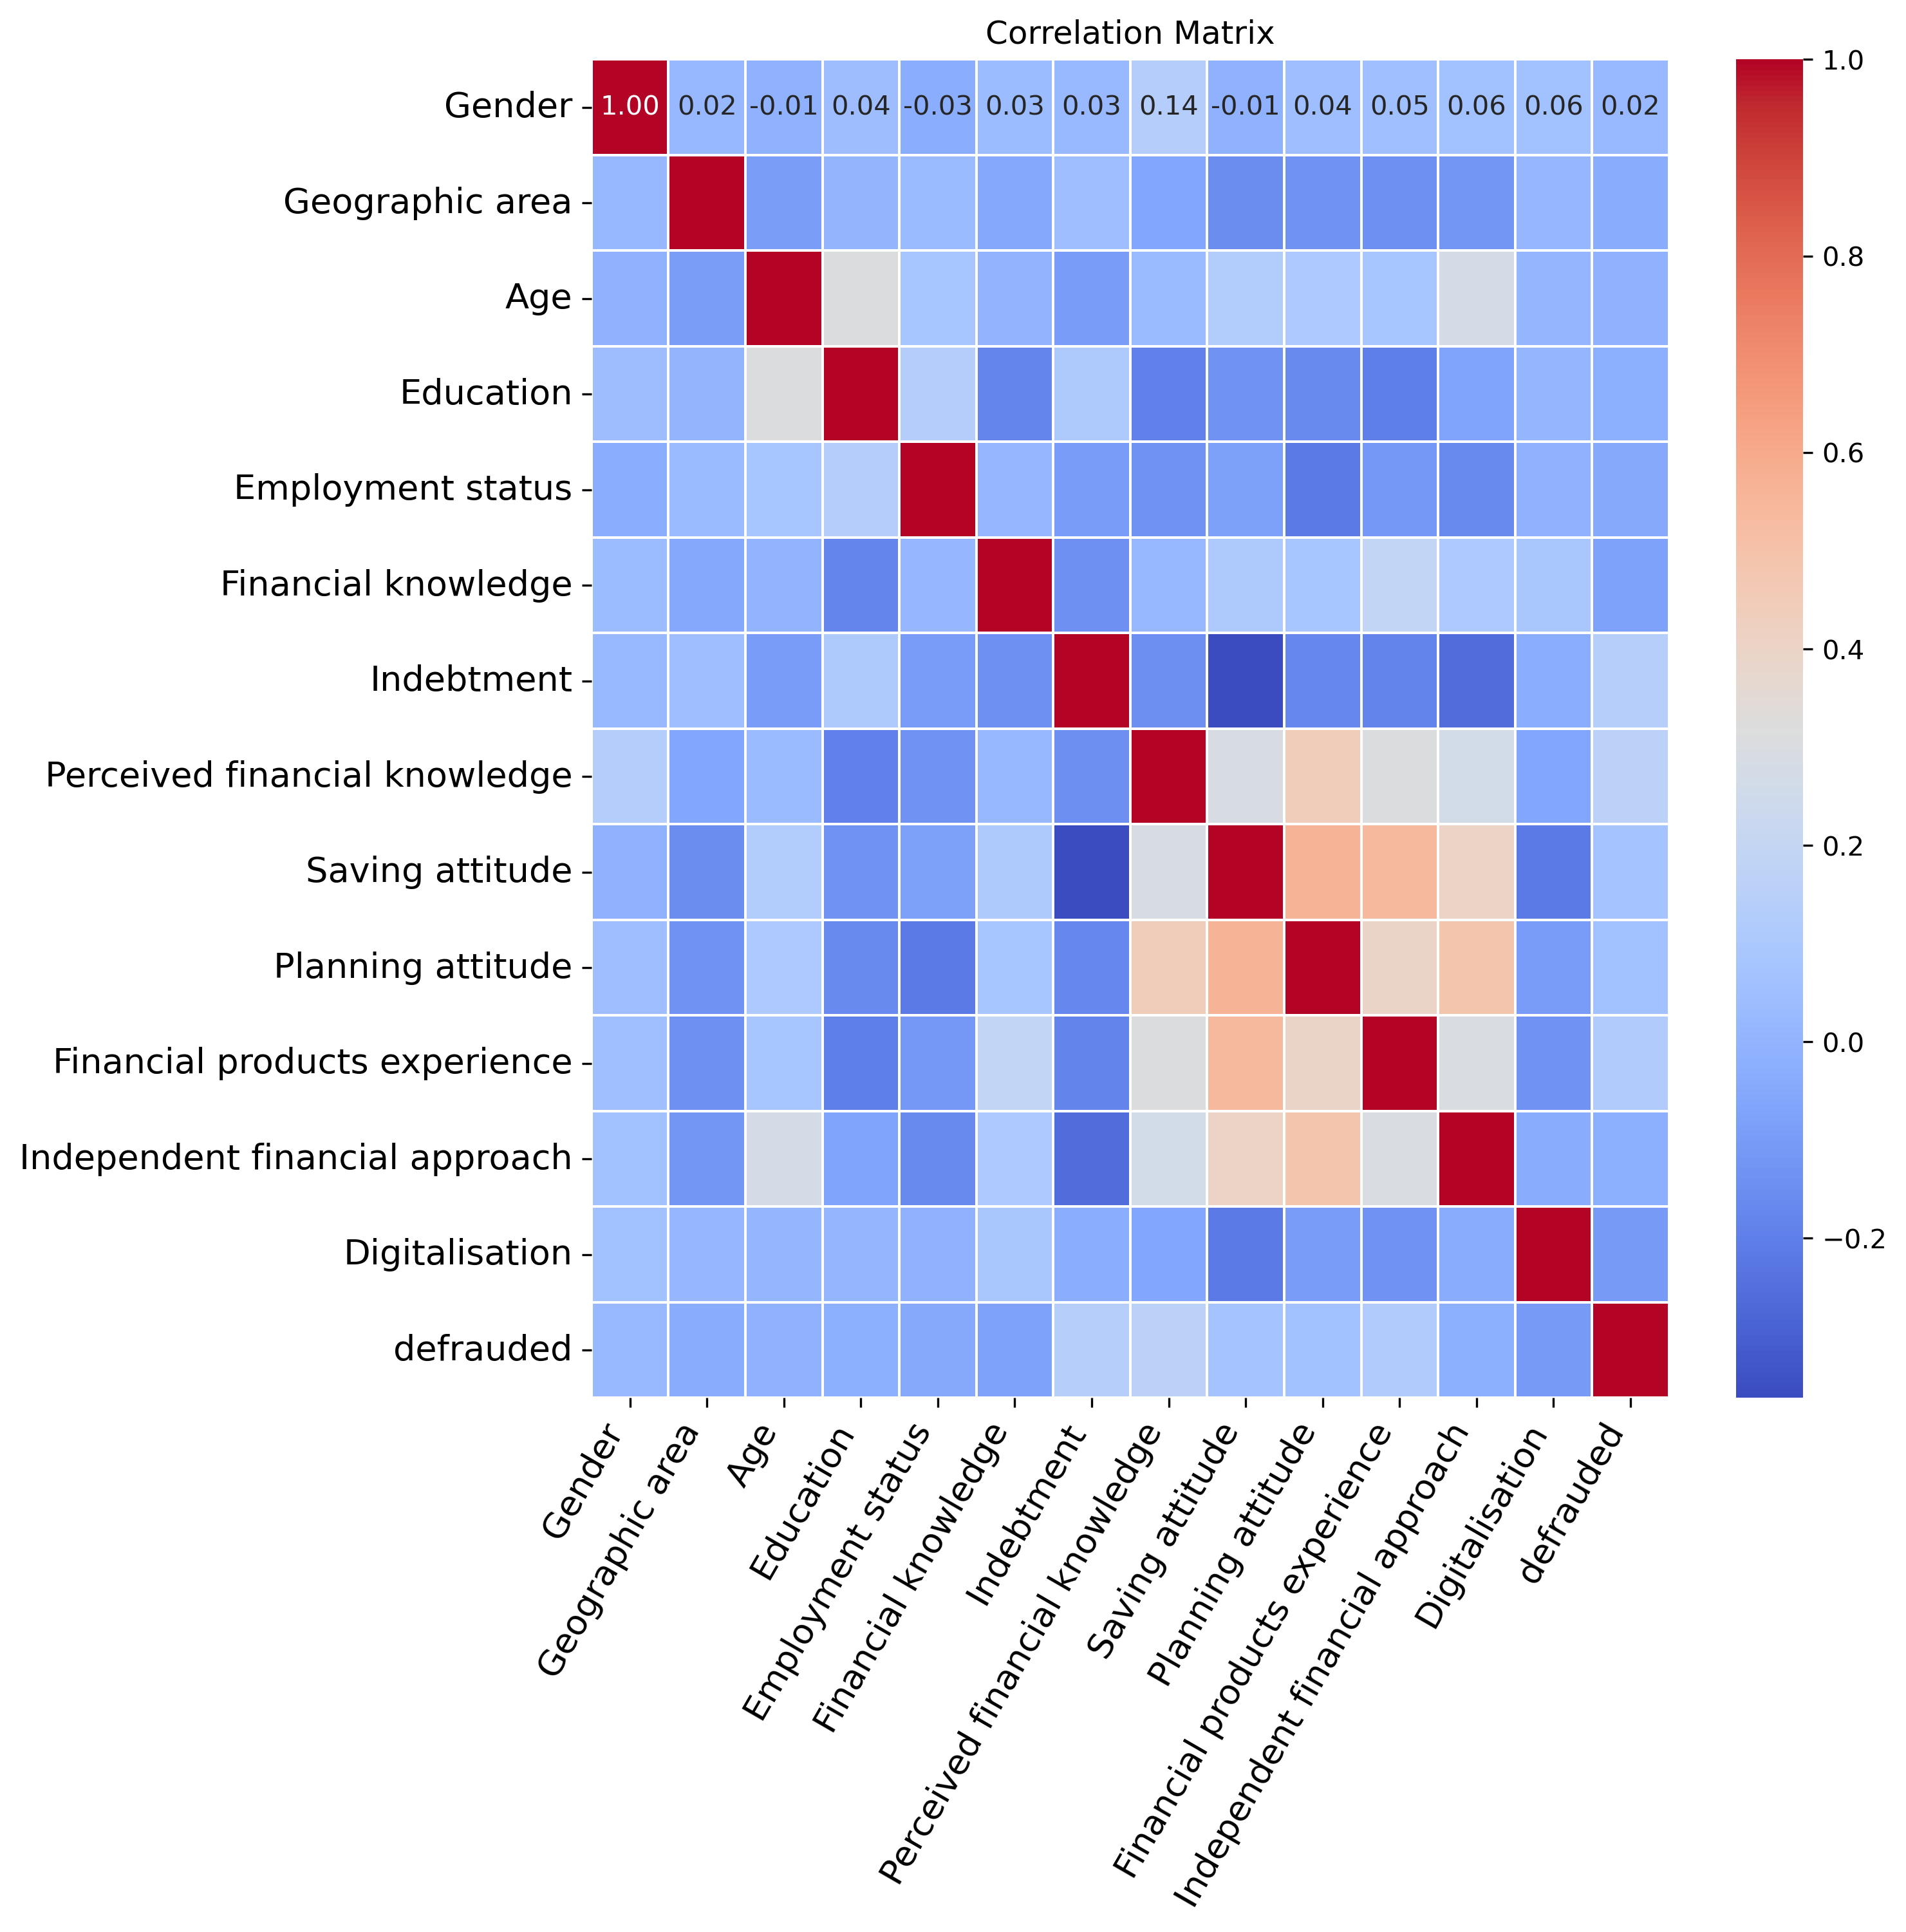
\includegraphics[width=13.85cm]{Corrplot.png}
	%\includegraphics[width=7cm]{imm/grafico_potenza.png}
        %\includegraphics[width=7cm]{imm/log_potenza.png}
	%\captionsetup{format=hang}
 \caption{Correlation matrix}
 \label{corr}
\end{figure}

\begin{figure}[H]
  \centering
        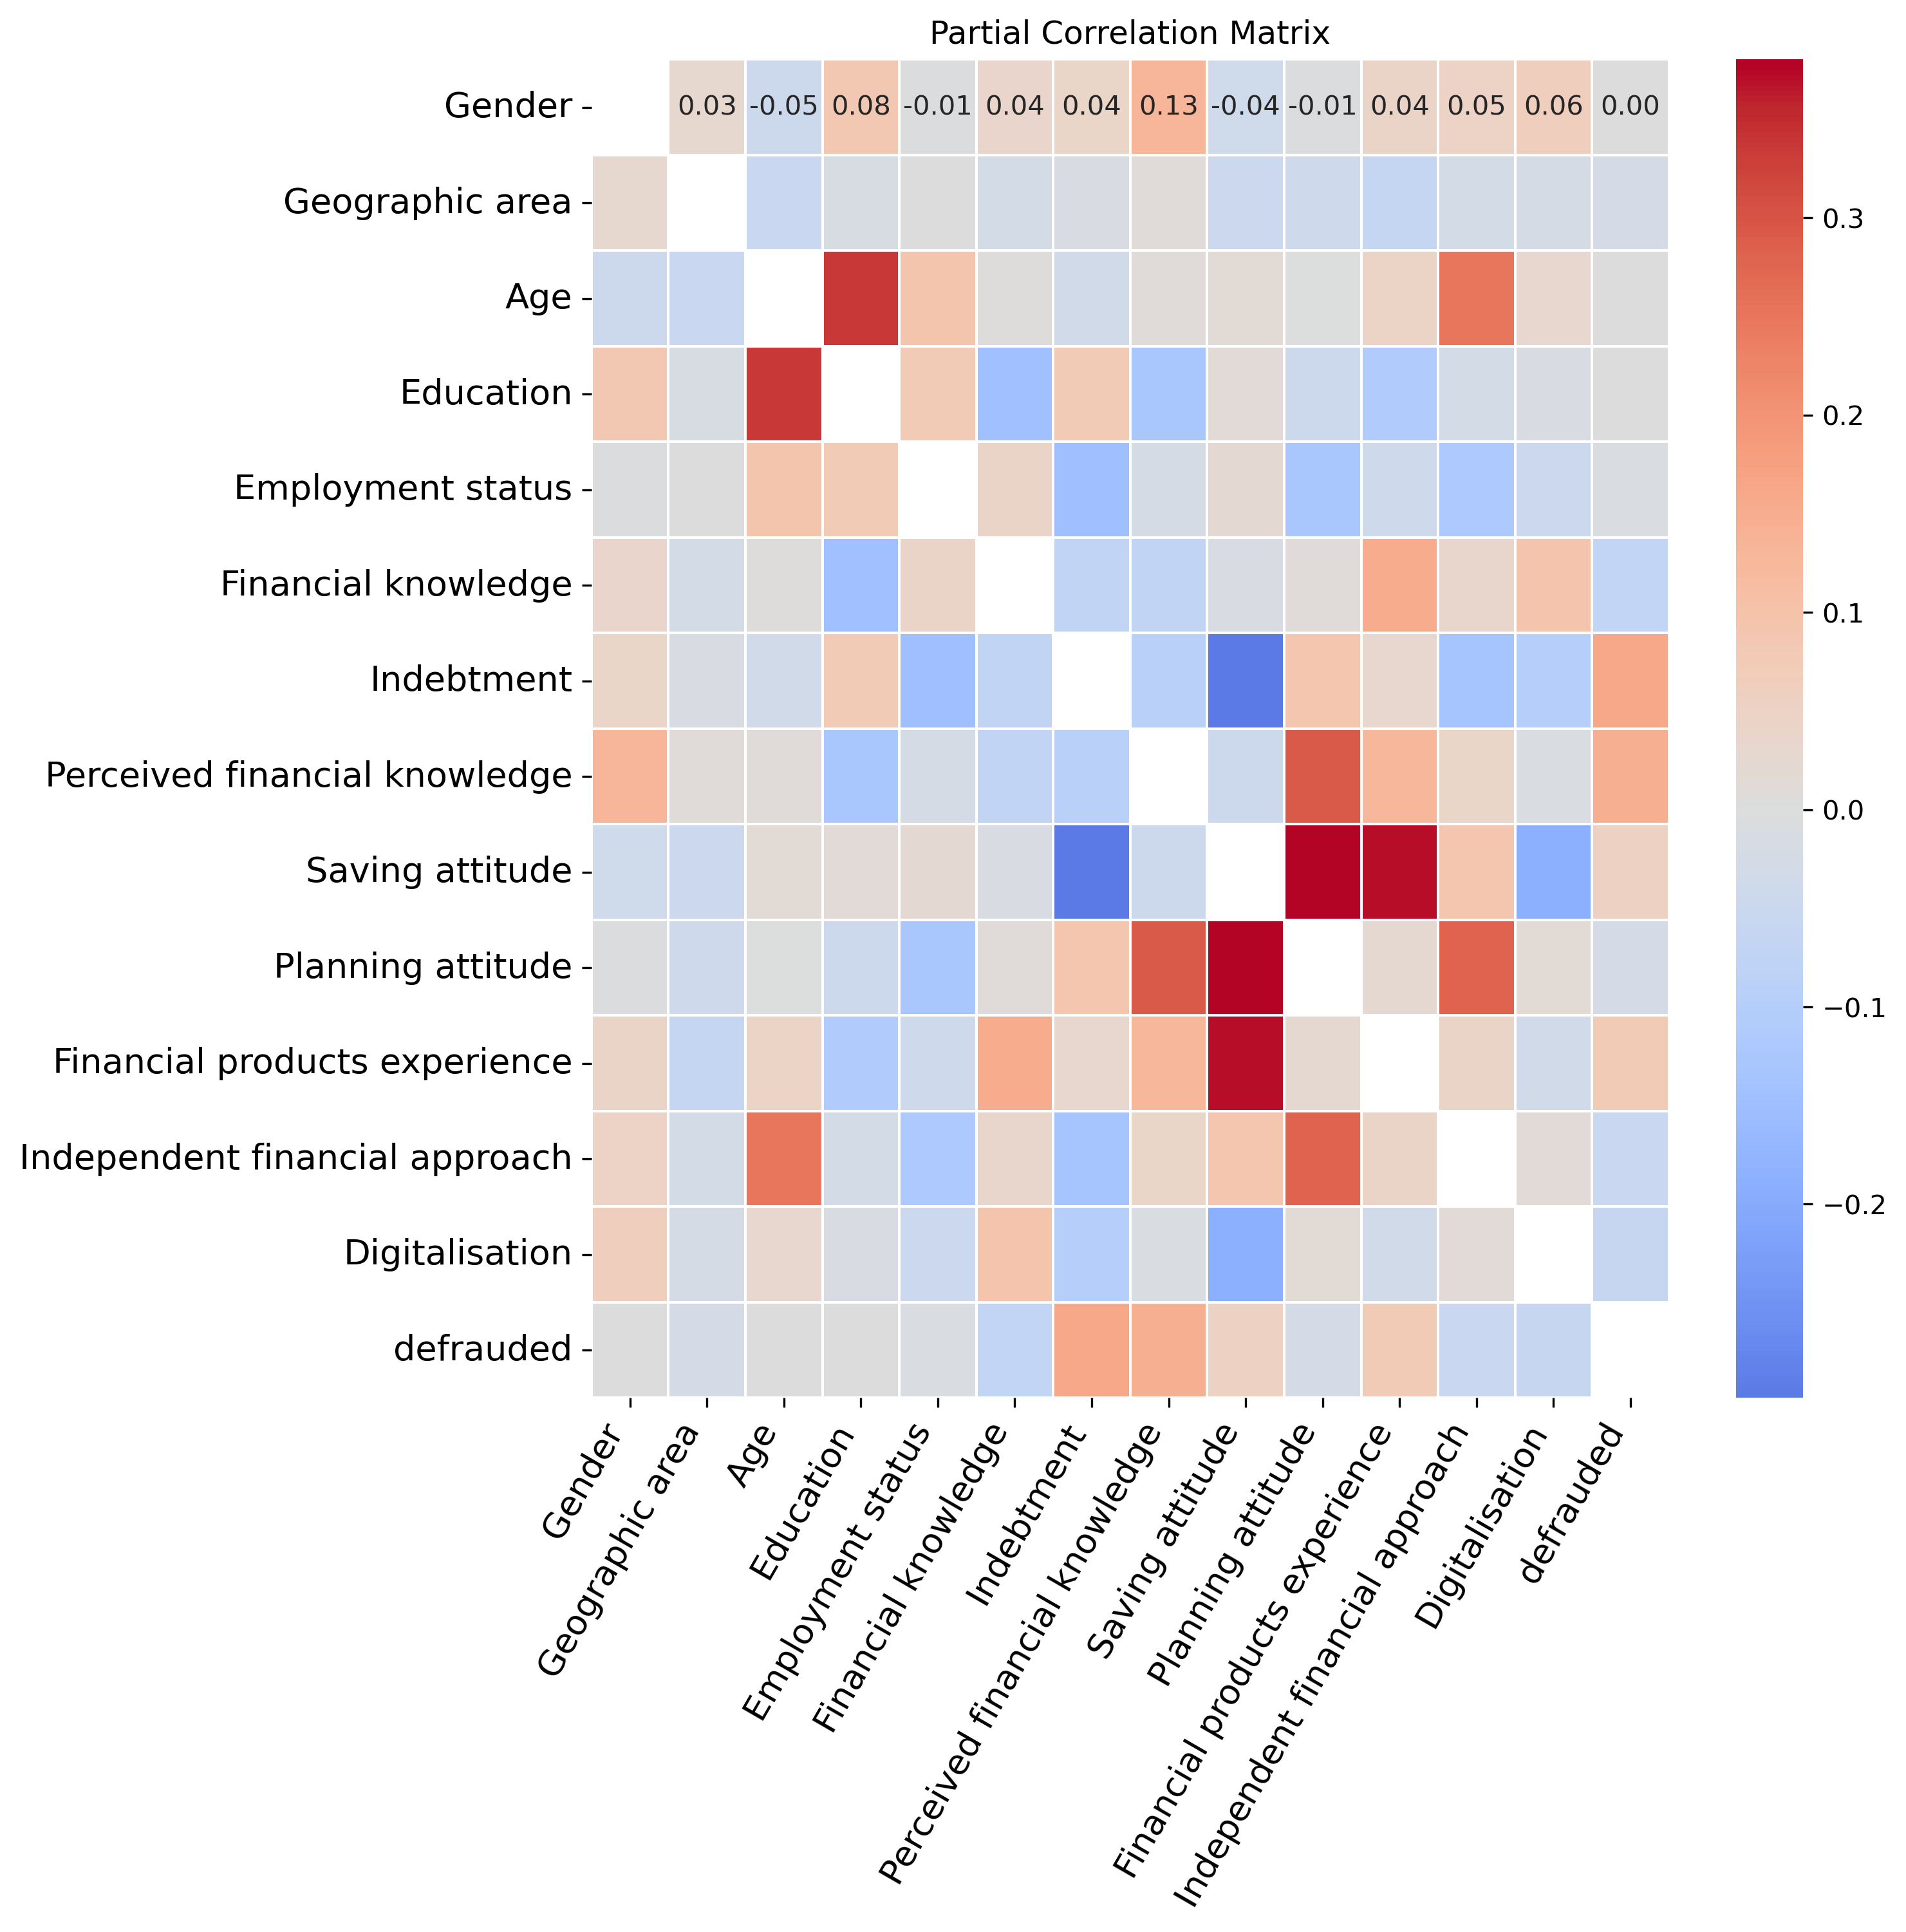
\includegraphics[width=13.85cm]{parcorrplot.png}
	%\includegraphics[width=7cm]{imm/grafico_potenza.png}
        %\includegraphics[width=7cm]{imm/log_potenza.png}
	%\captionsetup{format=hang}
 \caption{ Partial correlation matrix}
 \label{parcorr}
\end{figure}


Upon examination of the correlation matrices, it becomes evident that the main diagonal of the correlation matrix [Fig.\ref{corr}] is consistently equal to 1, as each variable is perfectly correlated with itself; in contrast, the partial correlation matrix [Fig.\ref{parcorr}] exhibits a diagonal with values equal to 0, which is a consequence of the removal of all its influence with itself. Furthermore, an area of distinction can be observed in the correlation matrix [Fig.\ref{corr}], differing in color from the overall matrix and representing the correlation between some of the features generated through feature engineering. It can be observed that the relationship between the features, which were created through the aforementioned process, is relatively neutral and generally more decorrelated than the others. This result demonstrates that the feature engineering process facilitated the generation of new features that are well-structured, independent of one another and highly informative with regard to the analysis context. In contrast, the partial correlation matrix [Fig.\ref{parcorr}] indicates a strong relationship between: 
\begin{itemize}
\item “\textit{Planning attitude}” and “\textit{Saving attitude}” which can be explained with the fact that saving usually implies planning and vice versa to a certain degree
\item “\textit{Financial products experience}” and “\textit{Saving attitude}” which can be explained thanks to the fact that to save in the digital age one is somewhat forced to open and use financial products
\item “\textit{Education}” and “\textit{Age}” which we can interpret through the lens that generally speaking younger people may have not yet completed their education
\item “\textit{Saving attitude}” and “\textit{Indebtment}” which we can explain thinking that in general being more of a spender often implies having more debt and having more savings implies generally speaking not having to resort to debt when facing difficulties 
\end{itemize}


\section{Data Analysis}

The most versatile and most useful classifiers of choice for our project are tree based models and the logistic regression, which keep explainability and are generally versatile in predicting a binary output, which in our case corresponds to predict if the respondent of the questionnaire has been a victim of a financial fraud. To be more precise, we decided to test three different classifiers:

\begin{itemize}
	\item \textit{Random Forest}, which is a collective learning method that exploits a committee of decision trees
	\item \textit{Logistic Regression}, which uses parametric conditional probability to assign new observations to one of the target’s class
	\item \textit{Multi-Layer Perceptron}, which is a specific case of the \textit{Artificial Neural Network}, composed by multiple hidden layers
\end{itemize}

We train these three classifiers based on the \textit{Matthews Correlation Coefficient} (MCC) \cite{BioData} \cite{BMC} as a measure of the quality of binary classification. The MCC takes into account true and false positives and negatives and is generally regarded as a balanced measure which can be used if the classes are of very different size, which is the case in our dataset. The MCC returns a value between -1 and +1 where +1 represents a perfect correlation between predicted and actual values, 0 no better than random prediction and -1 complete negative correlation between prediction and observation. 
The MCC can be directly calculated from the confusion matrix and we can find its value as:
\begin{equation}
	MCC = \frac{TP \cdot TN - FP \cdot FN}{\sqrt{(TP+FP)(TP+FN)(TN+FP)(TN+FN)}}
\end{equation}
where TP is the number of true positives, TN is the number of true negatives, FP is the number of false positives and FN is the number of false negatives. 

To get results that make more sense and are averaged over different partitions of the dataset without being case-specific, we decided to combine a cross-validation method with each classifier. The cross validation uses a different strategy to train and evaluate the analysis made; the number of \textit{k} folds you can use can vary, although the value we considered optimal for our case was 10. The dataset was divided into ten subsets and the three models were trained ten times. During each iteration, nine subsets served as the training set, while one subset functioned as the validation set. The validation set in each iteration is always a different one to prevent the same scenario to be recreated; this process facilitates a more robust comparison among all precedent models. 

We start our analysis doing a simple test and then we move on to implement some techniques trying solving the main problems of the dataset. In particular, the simplest thing we can do to combat imbalances across the dataset is try and balance class weights for Random Forest and Linear Regression. Moving forward, we implement more drastic changes such as undersampling with and without class weights. The last thing we do for a better results interpretation is to test the best model at which we arrive with both the whole dataset, but also the new dataset composed by the socio-demographic and the engineered features. Below we move to a better explanation with more details.

\subsection{Simple test}
The most simple test we can do is try and approach the problem with simply feeding a Random Forest model, a Logistic Regression model and a Multi Layer Perceptron model our cleaned dataset, without any feature engineering, and without any methods to combat the class imbalance we already know present, apart from stratification in dividing test and training set. 
This, as can be somewhat expected, yields very poor results: even through a 10-fold cross validation Random Forest achieves an MCC of basically zero, Multi Layer Perceptron around 0.1 and Logistic Regression around 0.17; the problem is the class imbalance, as highlighted by extremely low values of recall and precision for class 1 of our target variable in all three cases. It is interesting to notice that the overall predictive power is not bad as these metrics, given that the AUC for Random Forest is highest (around 0.84), while for Logistic Regression and Multi Layer Perceptron decreases to around 0.71 and 0.64. 
\subsection{Class weights}
One of the first approaches we can do, at least in the case of Random Forest and of Logistic Regression, is to train the model such that class 1 is way more important that class 0: the model is penalised more when making mistakes on class 1, and hence should learn more. We decided to keep a proportion of classes similar to the proportion of data in our dataset, that is penalising errors on class 1 twelve times more than what is done on class 0. 

This approach is not possible on Multi Layer Perceptron because of its structure, but it's not big problem, considering results do not particularly improve: we see in fact a slight rise of Random Forest to an MCC of around 0.1 and essentially no effect on Logistic Regression; moreover overall predictive power, measured trough AUC, generally stays the same as in simple test.
\subsection{Undersampling with no Class Weights}
Another, more drastic approach is to undersample our dataset: using a random undersampling function that essentially cuts the excess of samples of class 0 is indeed drastic, but completely eliminates by definition any imbalances. Moreover this approach is applicable to all three models we considered, as it is implemented at the train-test split level.

This time results do improve, and a lot: after the usual 10-fold cross validation, Random Forest improves to an astonishing 0.4 MCC, while Logistic Regression to a more modest 0.3 and Multi Layer Perceptron to a 0.2 value of MCC. Given the fact that the undersampling is done at the train-test split we also averaged over 50 different undersampled versions along with the usual 10-fold cross validation and we found that our scores did not change particularly, with an MCC of 0.40, 0.28 and 0.26 respectively for Random Forest, Logistic Regression and Multi Layer Perceptron. 
Loss of predictive power is to be expected when removing samples, and indeed AUC is less than before, but not considerably less: in fact, this can be seen in figure [Fig.\ref{ROC_under_noweights}].

\begin{figure}[H]
  \centering
        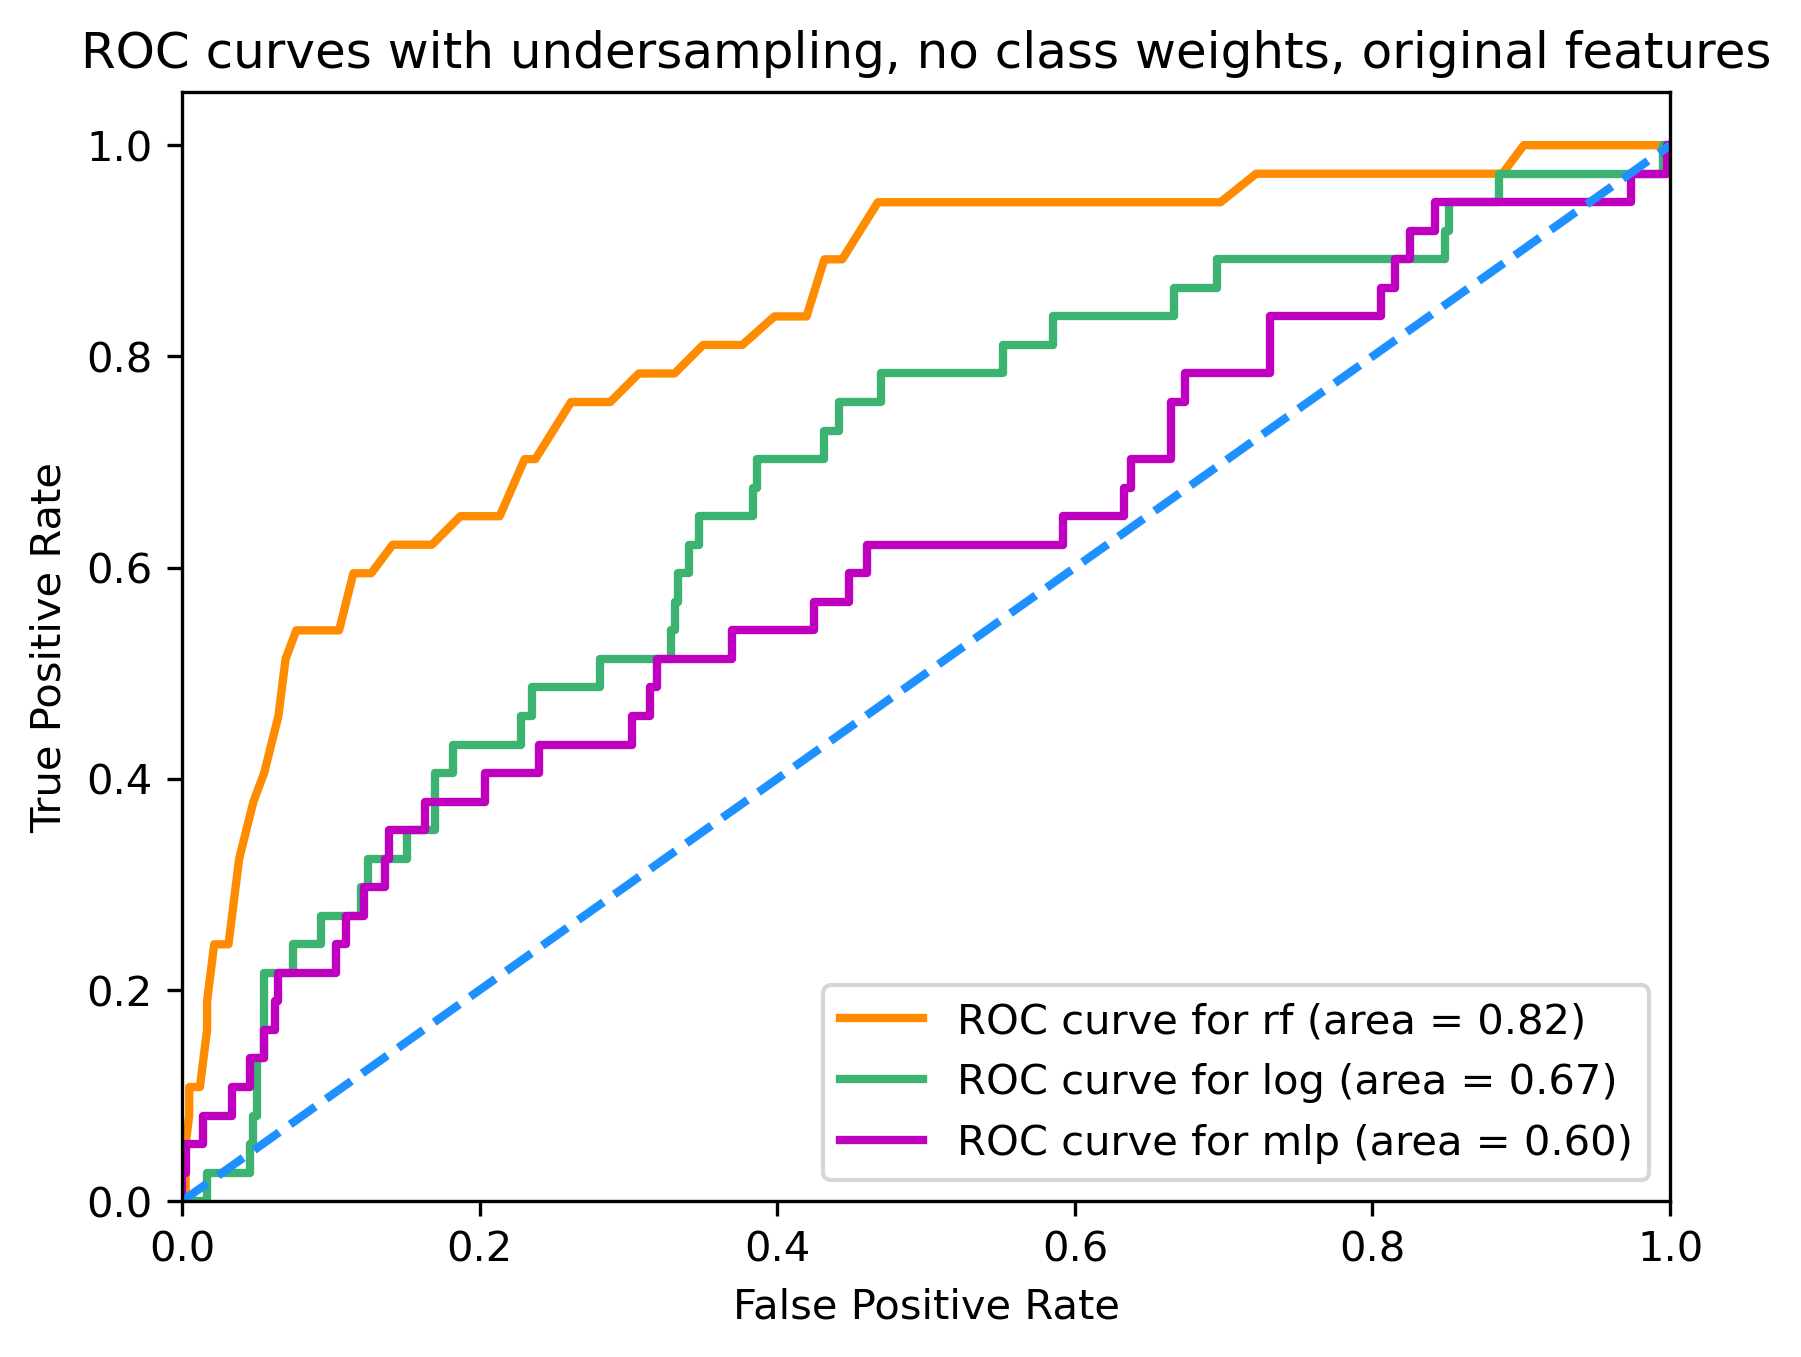
\includegraphics[width=10cm]{ROC_undersampling_noweights.png}
	%\includegraphics[width=7cm]{imm/grafico_potenza.png}
        %\includegraphics[width=7cm]{imm/log_potenza.png}
	%\captionsetup{format=hang}
 \caption{ROC curves of original features with undersampling and no class weights}
 \label{ROC_under_noweights}
\end{figure}

\subsection{Undersampling with Class Weights}
We can now try and combine both class weighting and undersampling; skipping already at the averaged and cross validated MCC scores we see that this time they actually do not improve, but rather they worsen from the case of just undersampling, with an MCC of 0.35, 0.13 and 0.25 respectively, signaling that uniting class weighting actually creates imbalances after the dataset had been undersampled exactly to combat imbalances. AUC is also impacted more negatively than before, as seen in figure [Fig.\ref{ROC_under_weights}]; note that clearly values for Multi Layer Perceptron stayed the same as it can't undergo class weighting.

\begin{figure}[H]
  \centering
        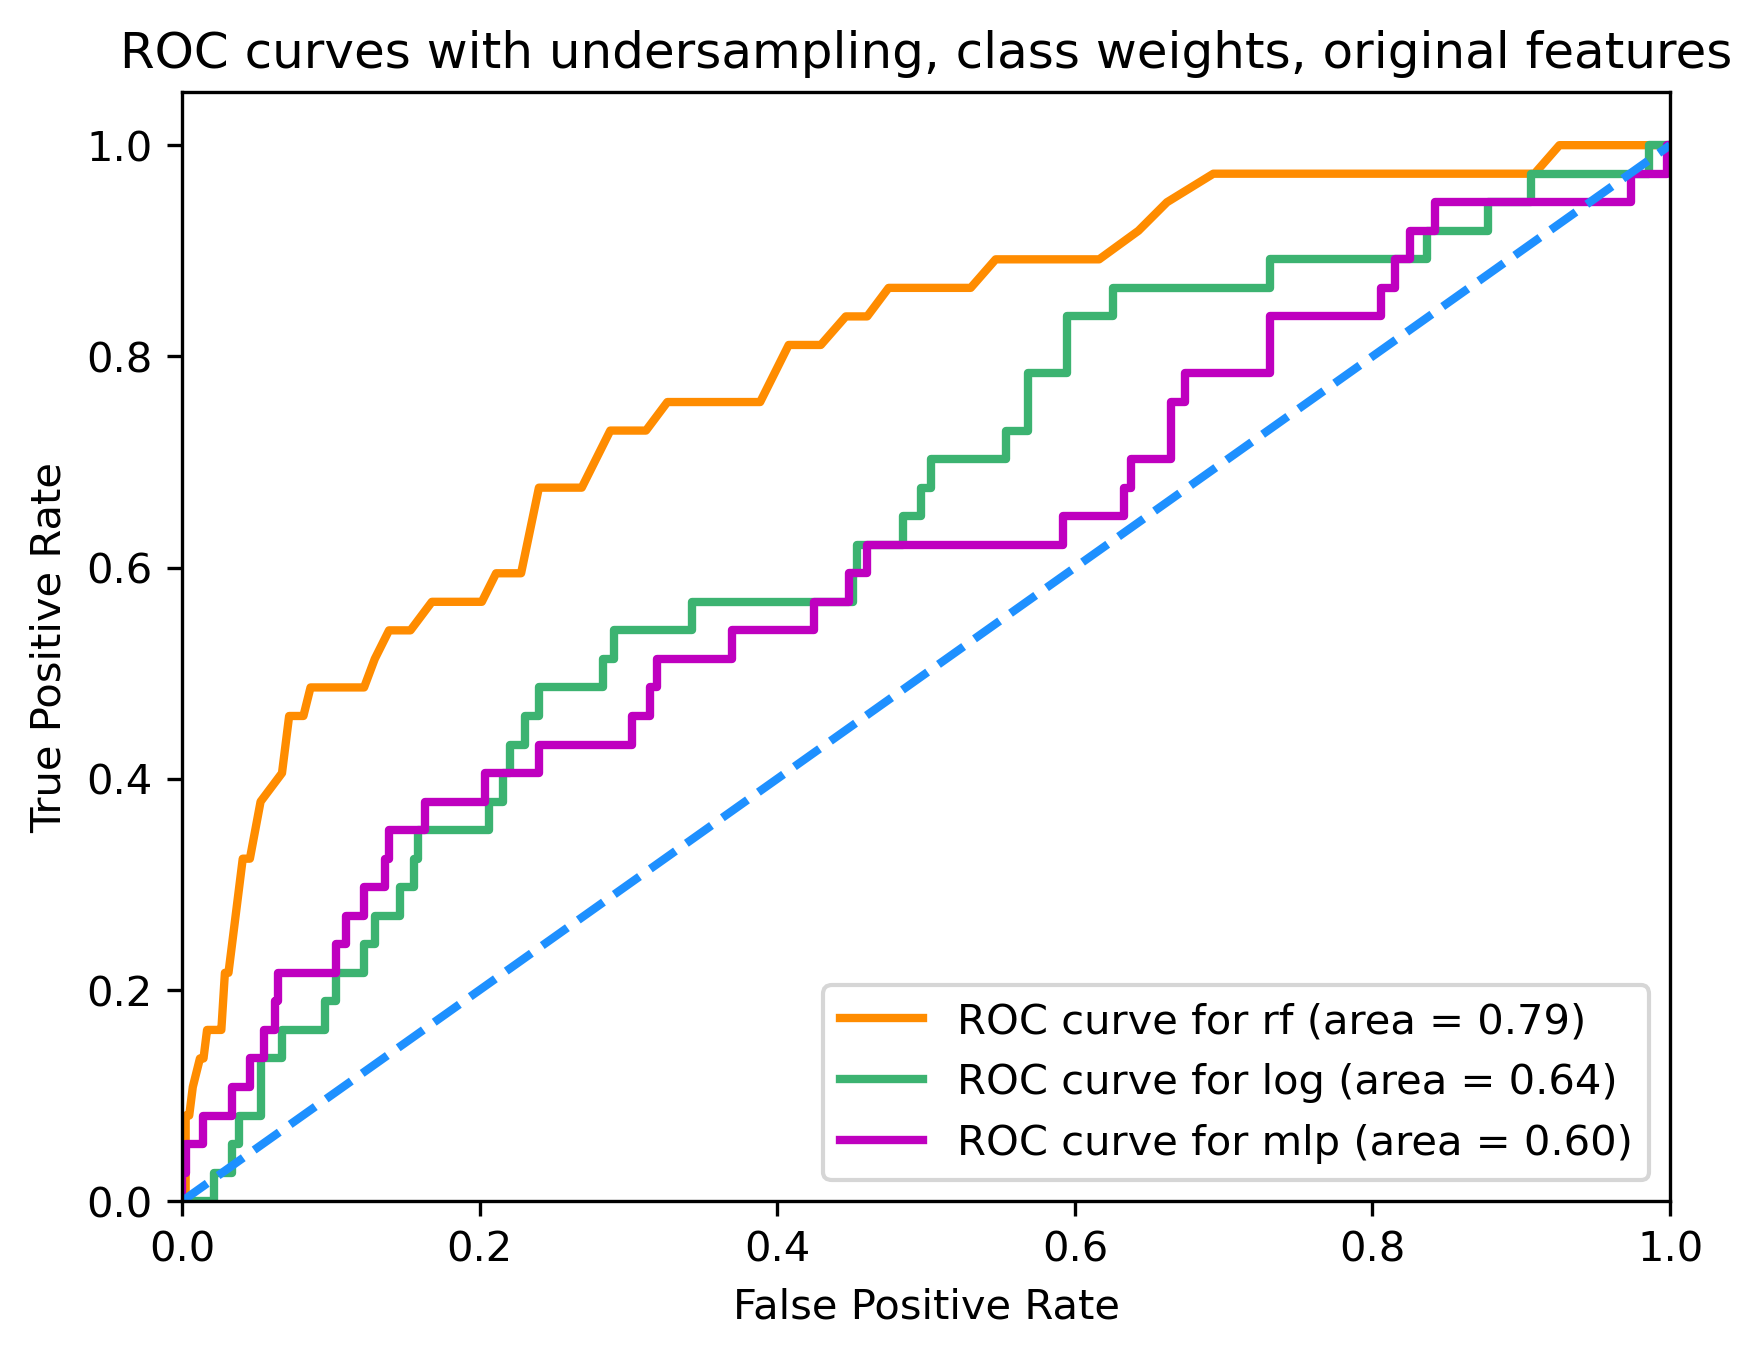
\includegraphics[width=10cm]{ROC_under_weights.png}
	%\includegraphics[width=7cm]{imm/grafico_potenza.png}
        %\includegraphics[width=7cm]{imm/log_potenza.png}
	%\captionsetup{format=hang}
 \caption{ROC curves of original features with undersampling and class weights}
 \label{ROC_under_weights}
\end{figure}

\subsection{Feature Engineering Impact}

At last, we have to ask ourselves if the process of feature engineering actually worsens our MCC and/or AUC; in general we can expect a loss in AUC but MCC should not vary too much as the dimensionality of the dataset is reduced and hence data points of interest are less sparse, albeit we lose information. We also know the new engineered features are uncorrelated with one another and so we can expect the model to not lose too much predictive power. For this analysis we'll consider only Random Forest with undersampling and no class weights, as it proved to be the best combination. With this configuration, the MCC is computed to be 0.35 when averaged over many undersampling iteration, with a slight decrease as expected, while AUC, depicted in figure [Fig.\ref{ROC_aggr_rf}] decreased a little to a mean value over iterations of 0.73, signaling that what was expected is found. 

\begin{figure}[H]
  \centering
        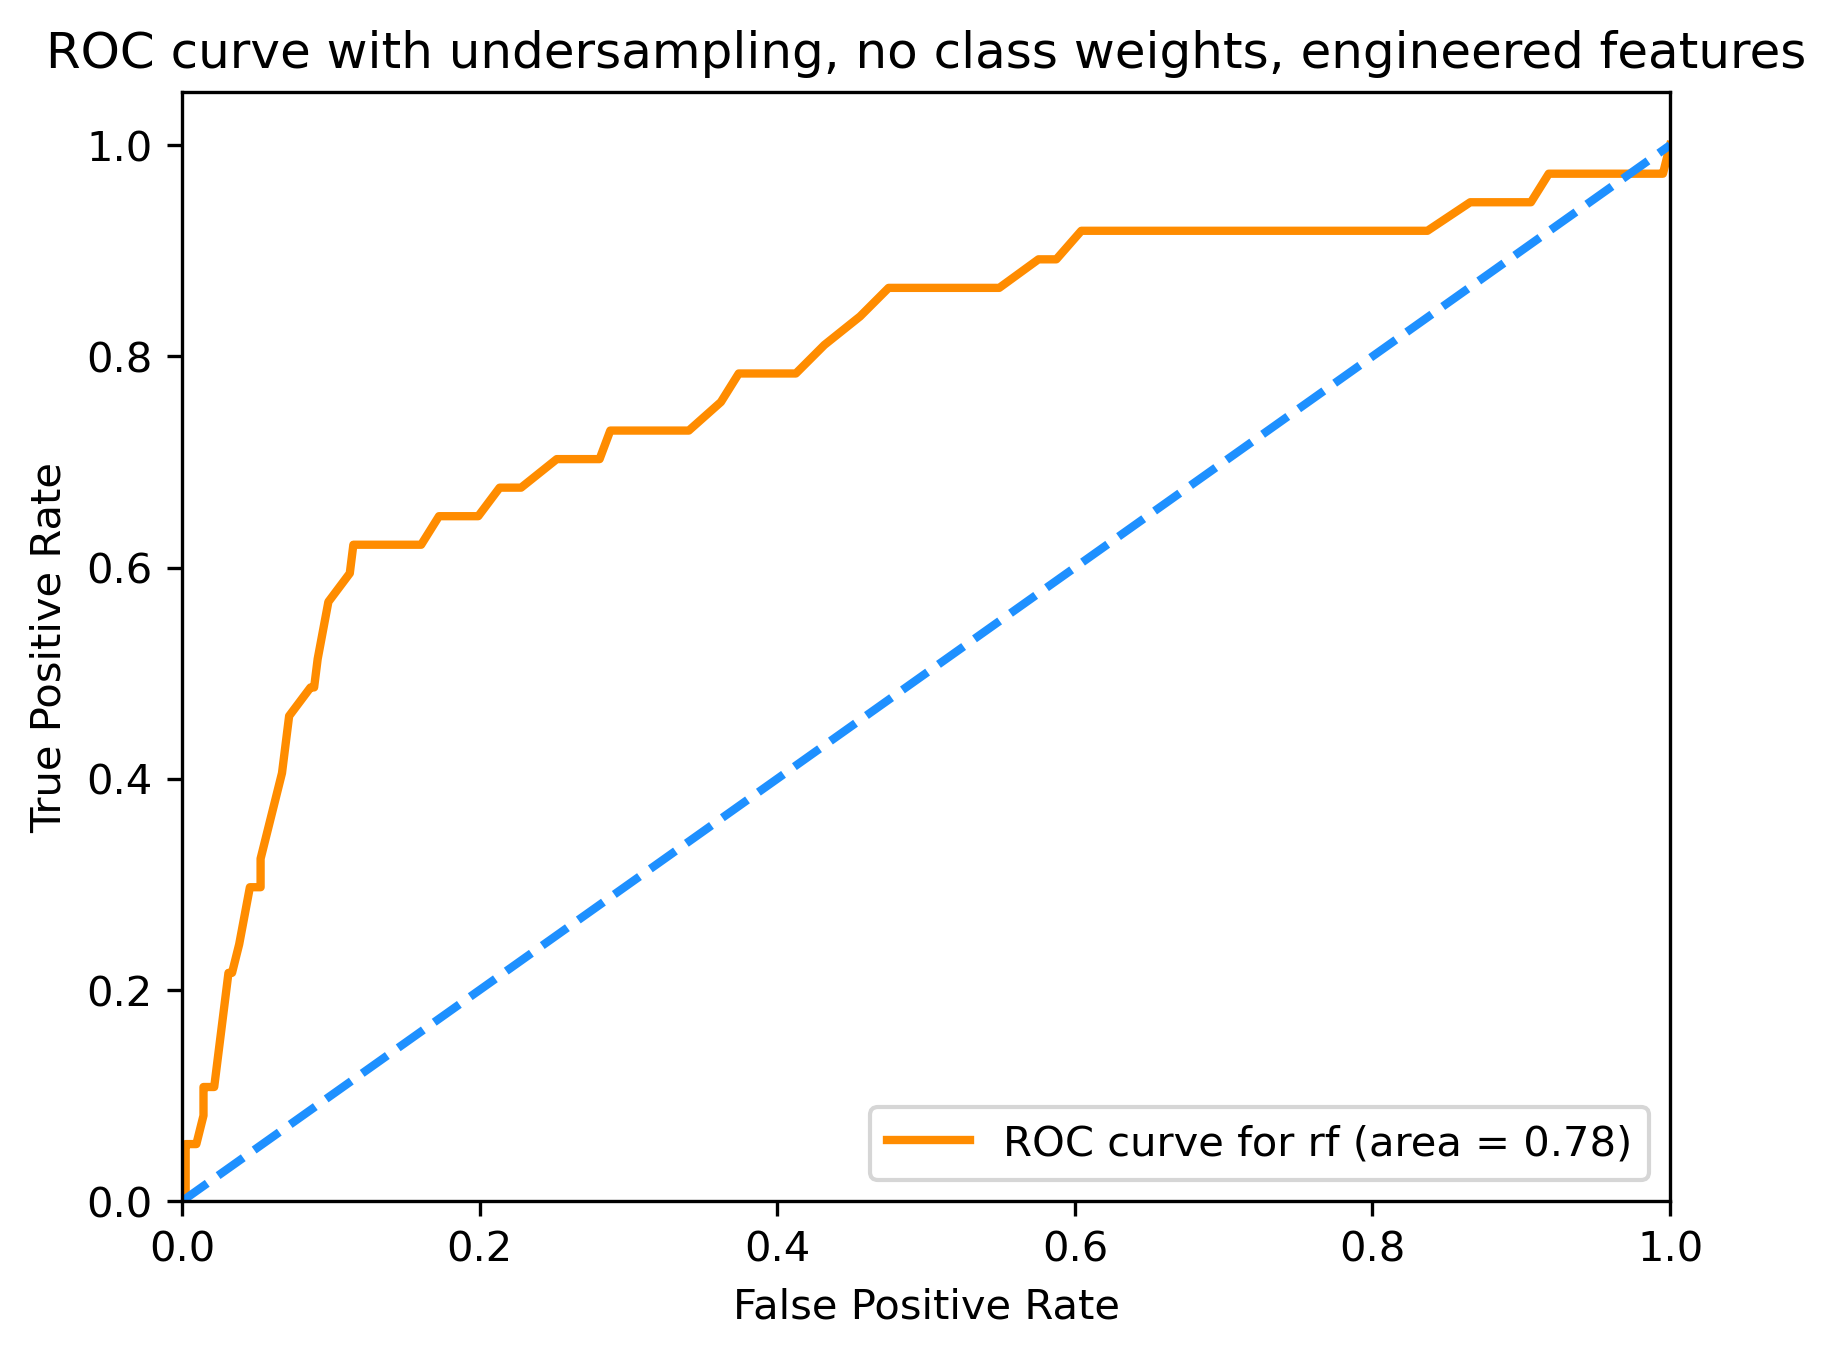
\includegraphics[width=10cm]{ROC_aggr_rf_under_noweights.png}
	%\includegraphics[width=7cm]{imm/grafico_potenza.png}
        %\includegraphics[width=7cm]{imm/log_potenza.png}
	%\captionsetup{format=hang}
 \caption{ROC curves of one iteration for engineered features with undersampling, no class weights}
 \label{ROC_aggr_rf}
\end{figure}

This means that for any result we can safely use as best model Random Forest with no class weights but with undersampling and applied to the engineered dataset, because the decrease in MCC and predictive power is small compared to the ease of interpretability within the dataset. This is optimal as it provides the best combination to perform feature selection while having an high level of interpretability.

\section{Results}
The first observation we do is related to the value of the MCC. In fact, one could argue that even a value of 0.35, which was the best we obtained, is not particularly high and that's true; but this has to be balanced with some arguments that must be taken into consideration. 

First things first, we know people are not always entirely truthful and/or precise; this is also especially true in Italy, where financial matters remain somewhat shrouded in a cloak of privacy and most of the time people feel attacked when asked questions in this sphere. This means that there will always be some systematic error given by these inconsistencies, and this error resulted at the start of the dataset in us losing some data points, but also later it can introduce quite some noise. This means an MCC close to 1 may never be obtained, and we have to aim lower; estimating the effects of this noise is an even harder task though. 

Then, the imbalance of the dataset and its high dimensionality definetly do not help. Computing some more metrics on our latest Random Forest model we see that we have, for our class of interest, values of 0.66, 0.68 and 0.65 for mean F1 score, mean precision and mean recall. These values indicate that generally speaking we have achieved a good tradeoff with predictive power and interpretability and explainability, which was what we were aiming for in the first place. 

At last, to some degree we also have to probably recognise that being fraud victims, contrary to popular belief, is an element of society that is transversal, that is can happen to everyone, and everyone has to be ready and prepared for when the time comes. 


We now want to aim at identifying any pattern that might be linked to being victims of a financial fraud in the contest of the stereotypical features we engineered and to do so we start with a simple feature importance with Gini entropy decrease. Since it does not take into account collinearity within features, we double check using Permutation Importance and compare the results. Analysed the importance of each feature, we investigate the impact each feature has on the target variable with Partial Dependences evaluating whether the findings align with the collective imagination or deviate from conventional wisdom. Lastly, we try to create some stereotypical profiles of people who might have replied to our survey to check what is the probability of them to being defrauded to compare it to common thought and to provide a somewhat practical example.

All these analyses will be done on a Random Forest model with undersampling, no class weights, trained on the engineered features' dataset.
More details on the results found are described in the following sections.


\subsection{Feature Importance}

The first analysis that is very classical and can be done is looking at the importance of each feature through the Gini index; this method is based on the decrease in impurity (e.g., Gini impurity or entropy) that each feature causes when used to split a node in the decision trees. The importance of a feature is calculated as the total reduction in the impurity across all trees in the forest, averaged over all trees. This is what is present in figure [Fig.\ref{Gini}].
\begin{figure}[H]
  \centering
        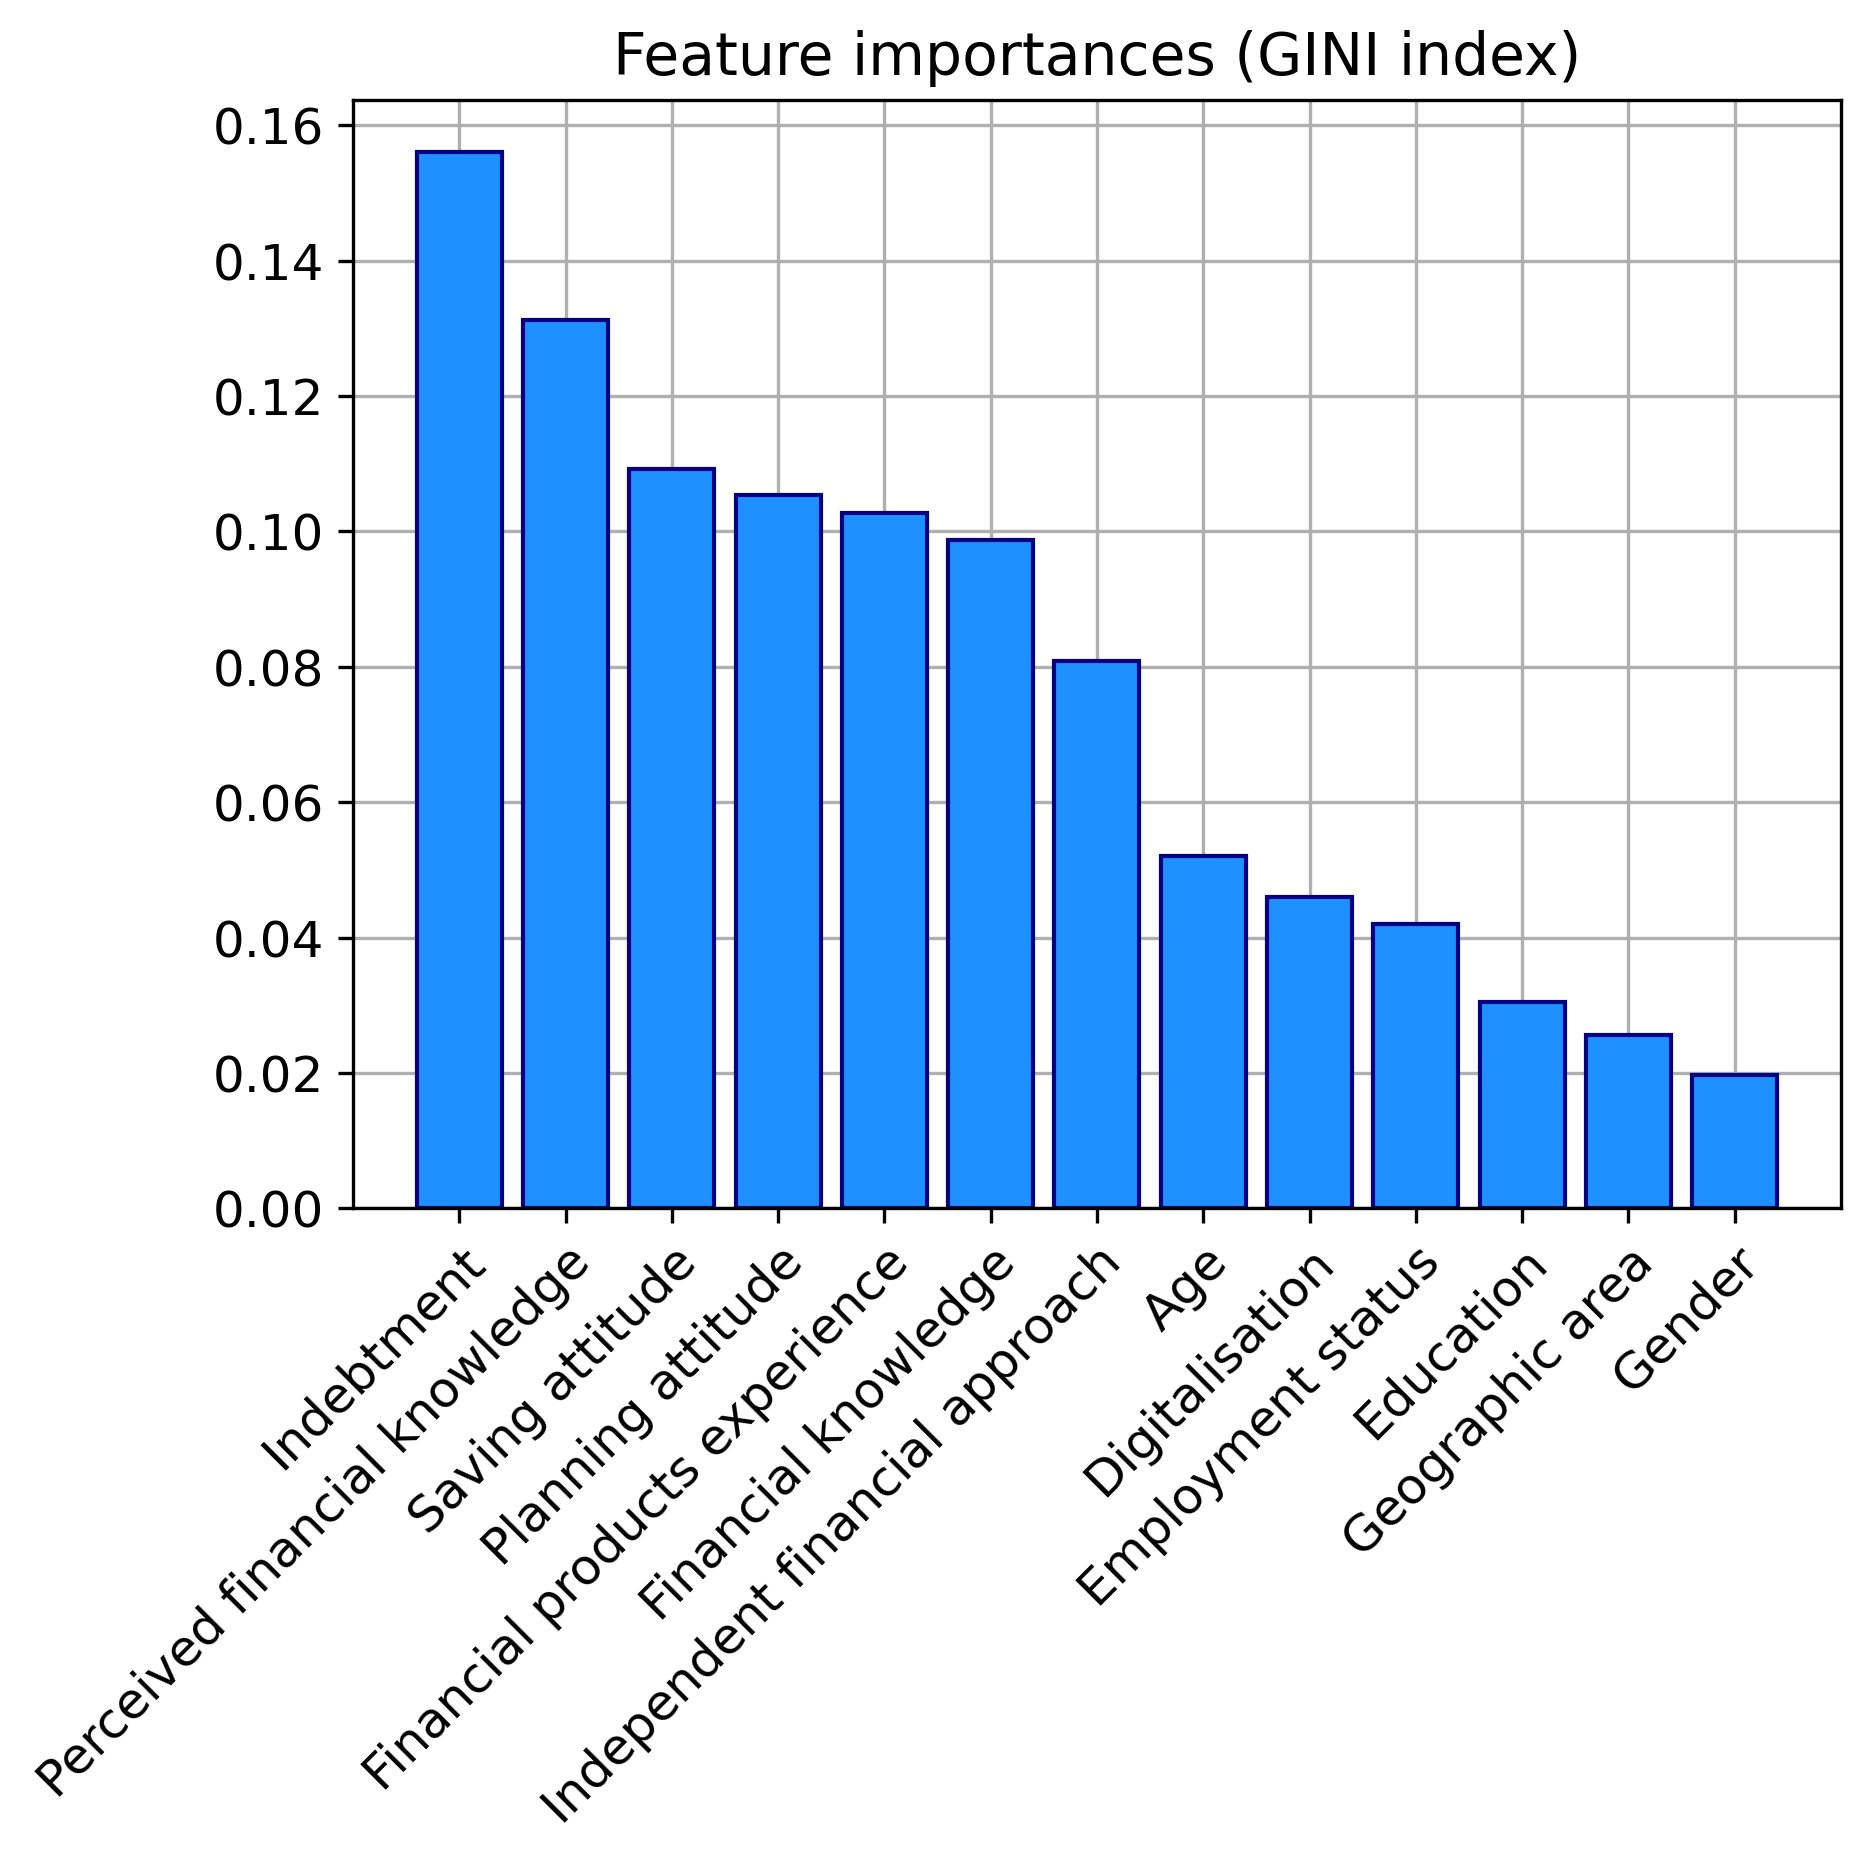
\includegraphics[width=12cm]{Gini_importance.png}
	%\includegraphics[width=7cm]{imm/grafico_potenza.png}
        %\includegraphics[width=7cm]{imm/log_potenza.png}
	%\captionsetup{format=hang}
 \caption{Feature importance considering Gini entropy decrease}
 \label{Gini}
\end{figure}


It's interesting to notice how, for our model, the most important attributes were all of the financial type, and not socio-demographic characteristics or tendencies such as digitalisation approach. 


Now to double check we also take a look at feature importance through permutation, in figure [Fig.\ref{permut}].

Permutation importance works in a fundamentally different way than Gini importance. The idea is that per each feature it shuffles its values in the dataset. This breaks the association between that feature and the target variable while keeping the other features the same; the idea is to simulate a situation where the feature provides no useful information to the model. Then it re-evaluates the model on the same test set; the drop in performance is calculated, indicating how important the feature was. A large drop in performance means the feature was important, while a small or no drop means the feature was not important.

\begin{figure}[H]
  \centering
        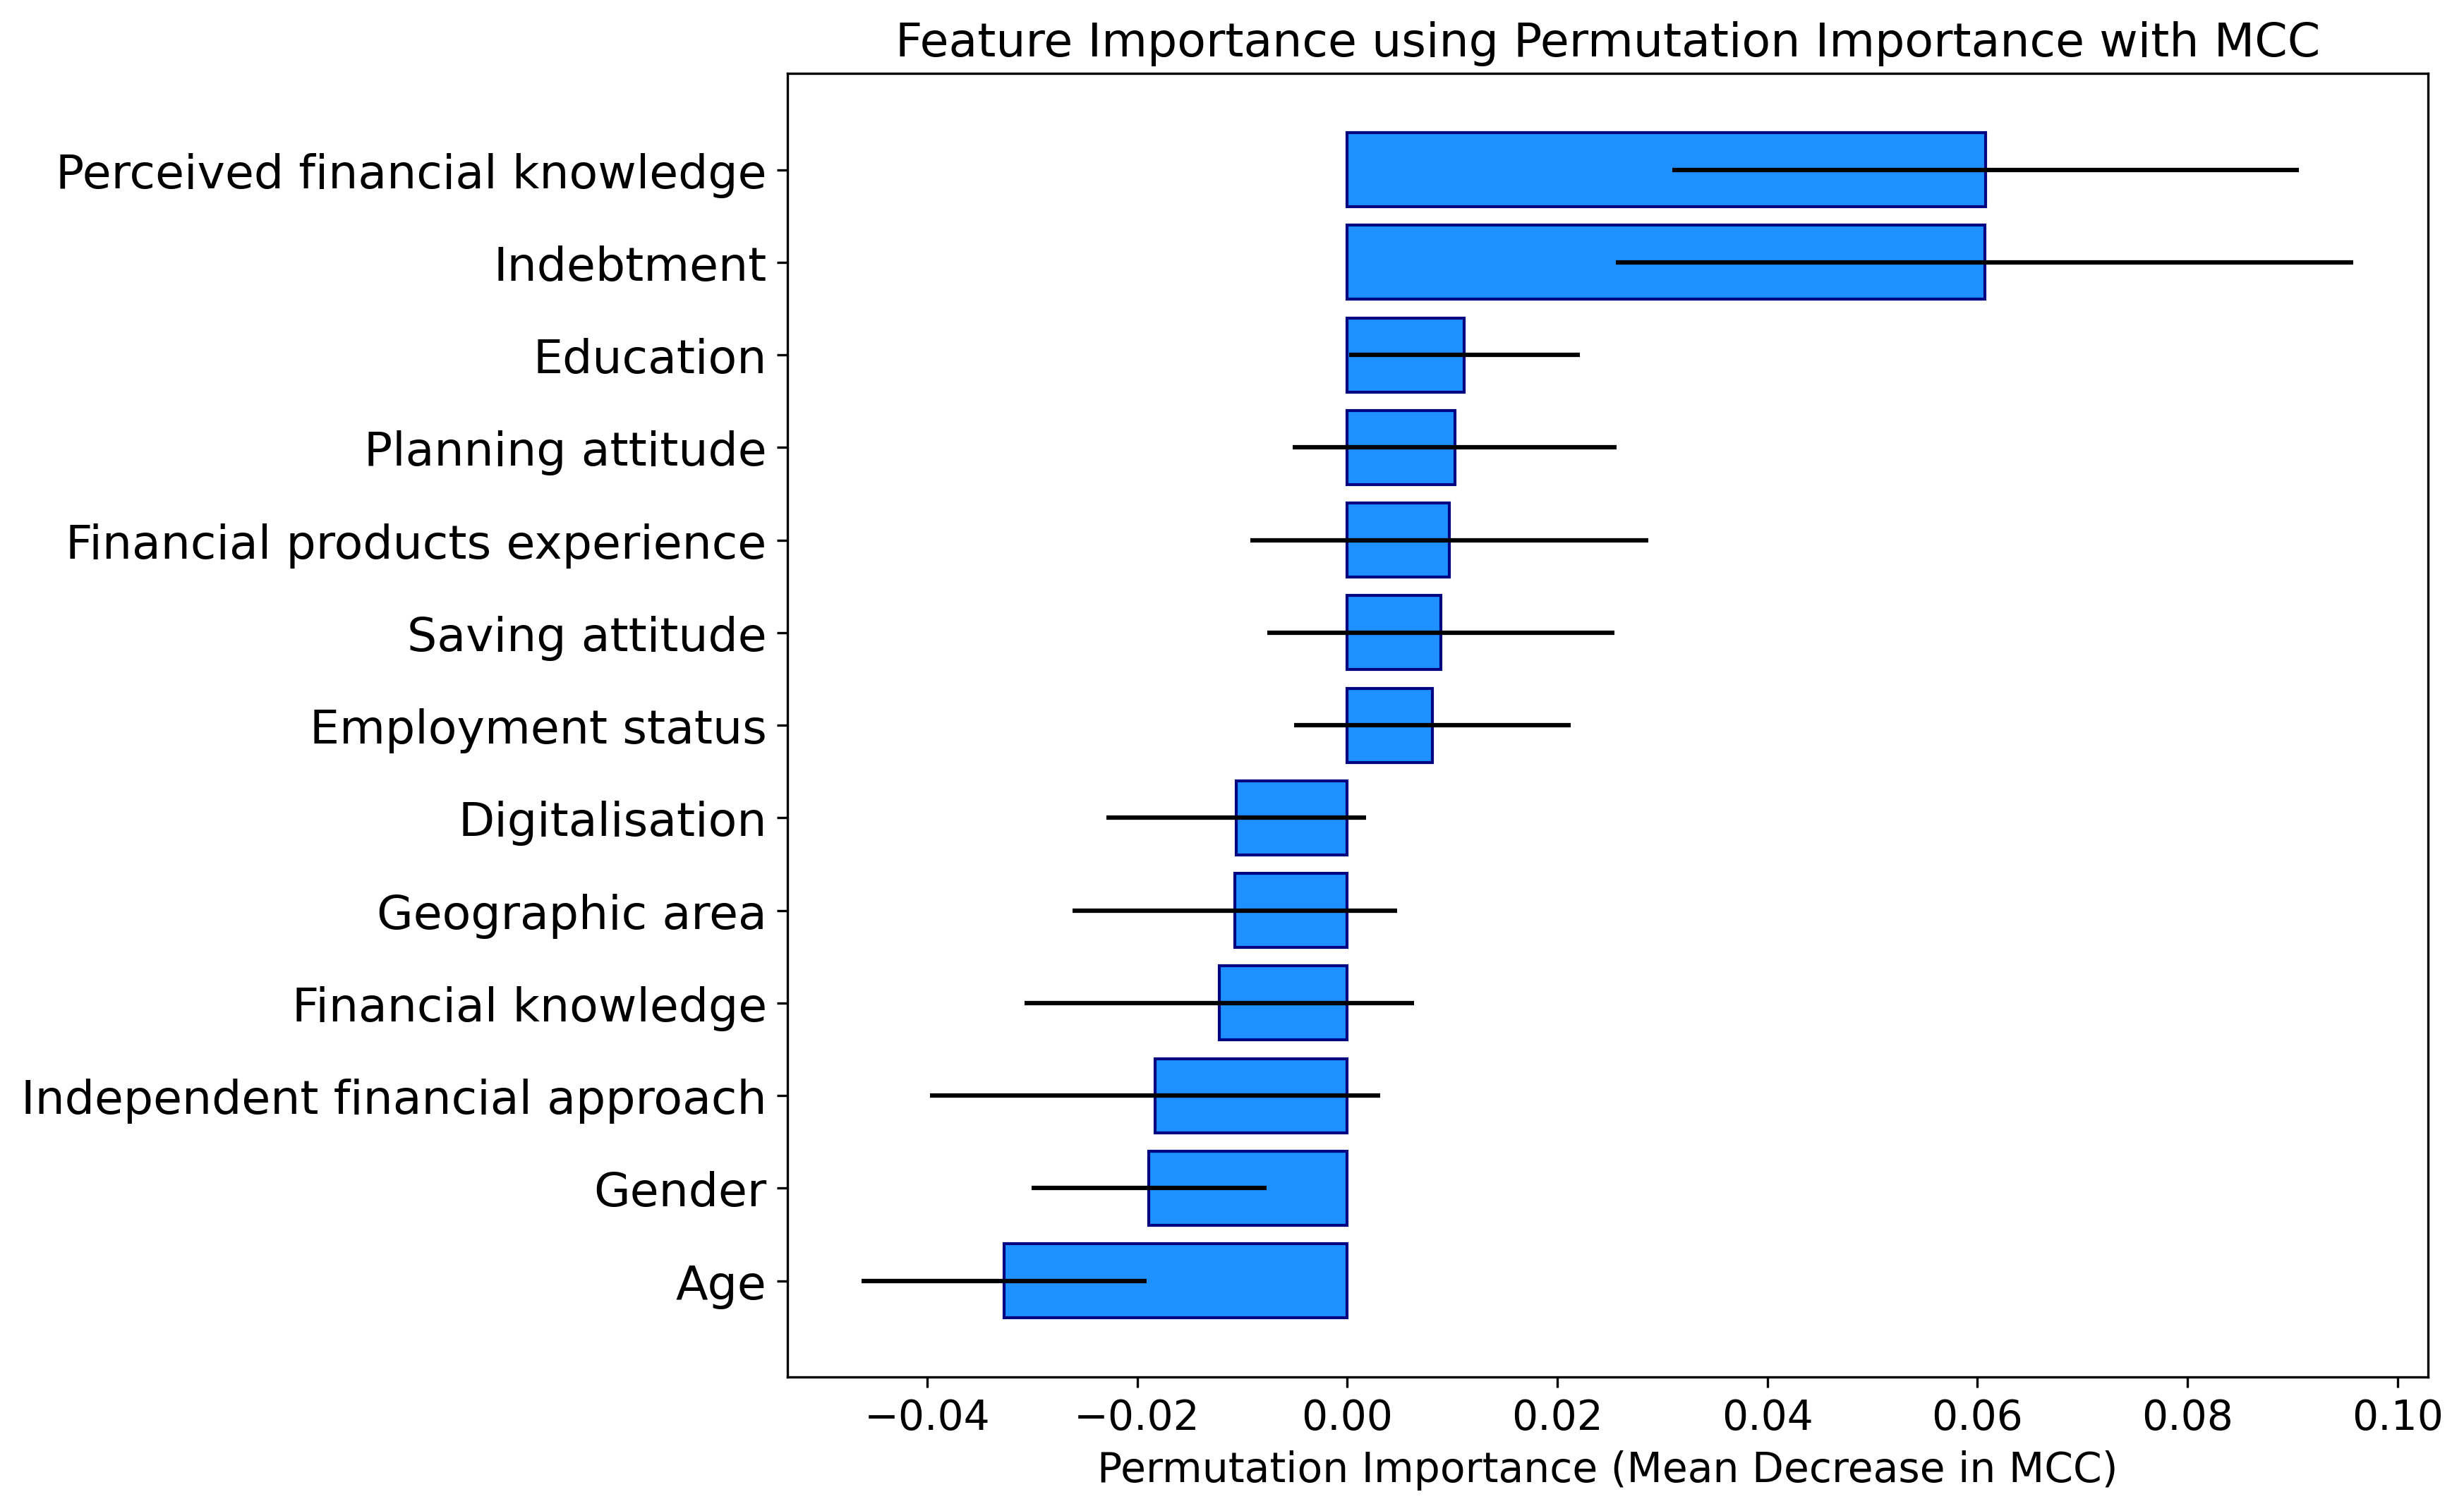
\includegraphics[width=14cm]{Permutation_importance.png}
	%\includegraphics[width=7cm]{imm/grafico_potenza.png}
        %\includegraphics[width=7cm]{imm/log_potenza.png}
	%\captionsetup{format=hang}
 \caption{Feature importance considering feature permutation}
 \label{permut}
\end{figure}

This time we can see that the two most important features were, within error bars,  \textit{``Perceived financial knowledge"} and \textit{``Indebtment"}, which were also the top two in Gini importance; conversely, we once again see that socio-demographic variables such as \textit{``Age"} and \textit{``Gender"} are not important; we also see that probably \textit{``Financial knowledge"} and \textit{``Independent financial approach"} exhibit collinearity with other variables, given that their specific importance is lower than what was present in the Gini plot. 

\subsection{Feature Partial Dependence with Target Variable}

As a more in depth analysis, we evaluate the influence of each characteristic on the target variable, taking partial dependencies into account. This will enable us to ascertain whether the results are in line with the collective imagination or deviate from conventional wisdom. The plots in figure [Fig.\ref{partialdep}] show the 13 possible combination between each feature and the defrauded feature.

\begin{figure}[H]
  \centering
        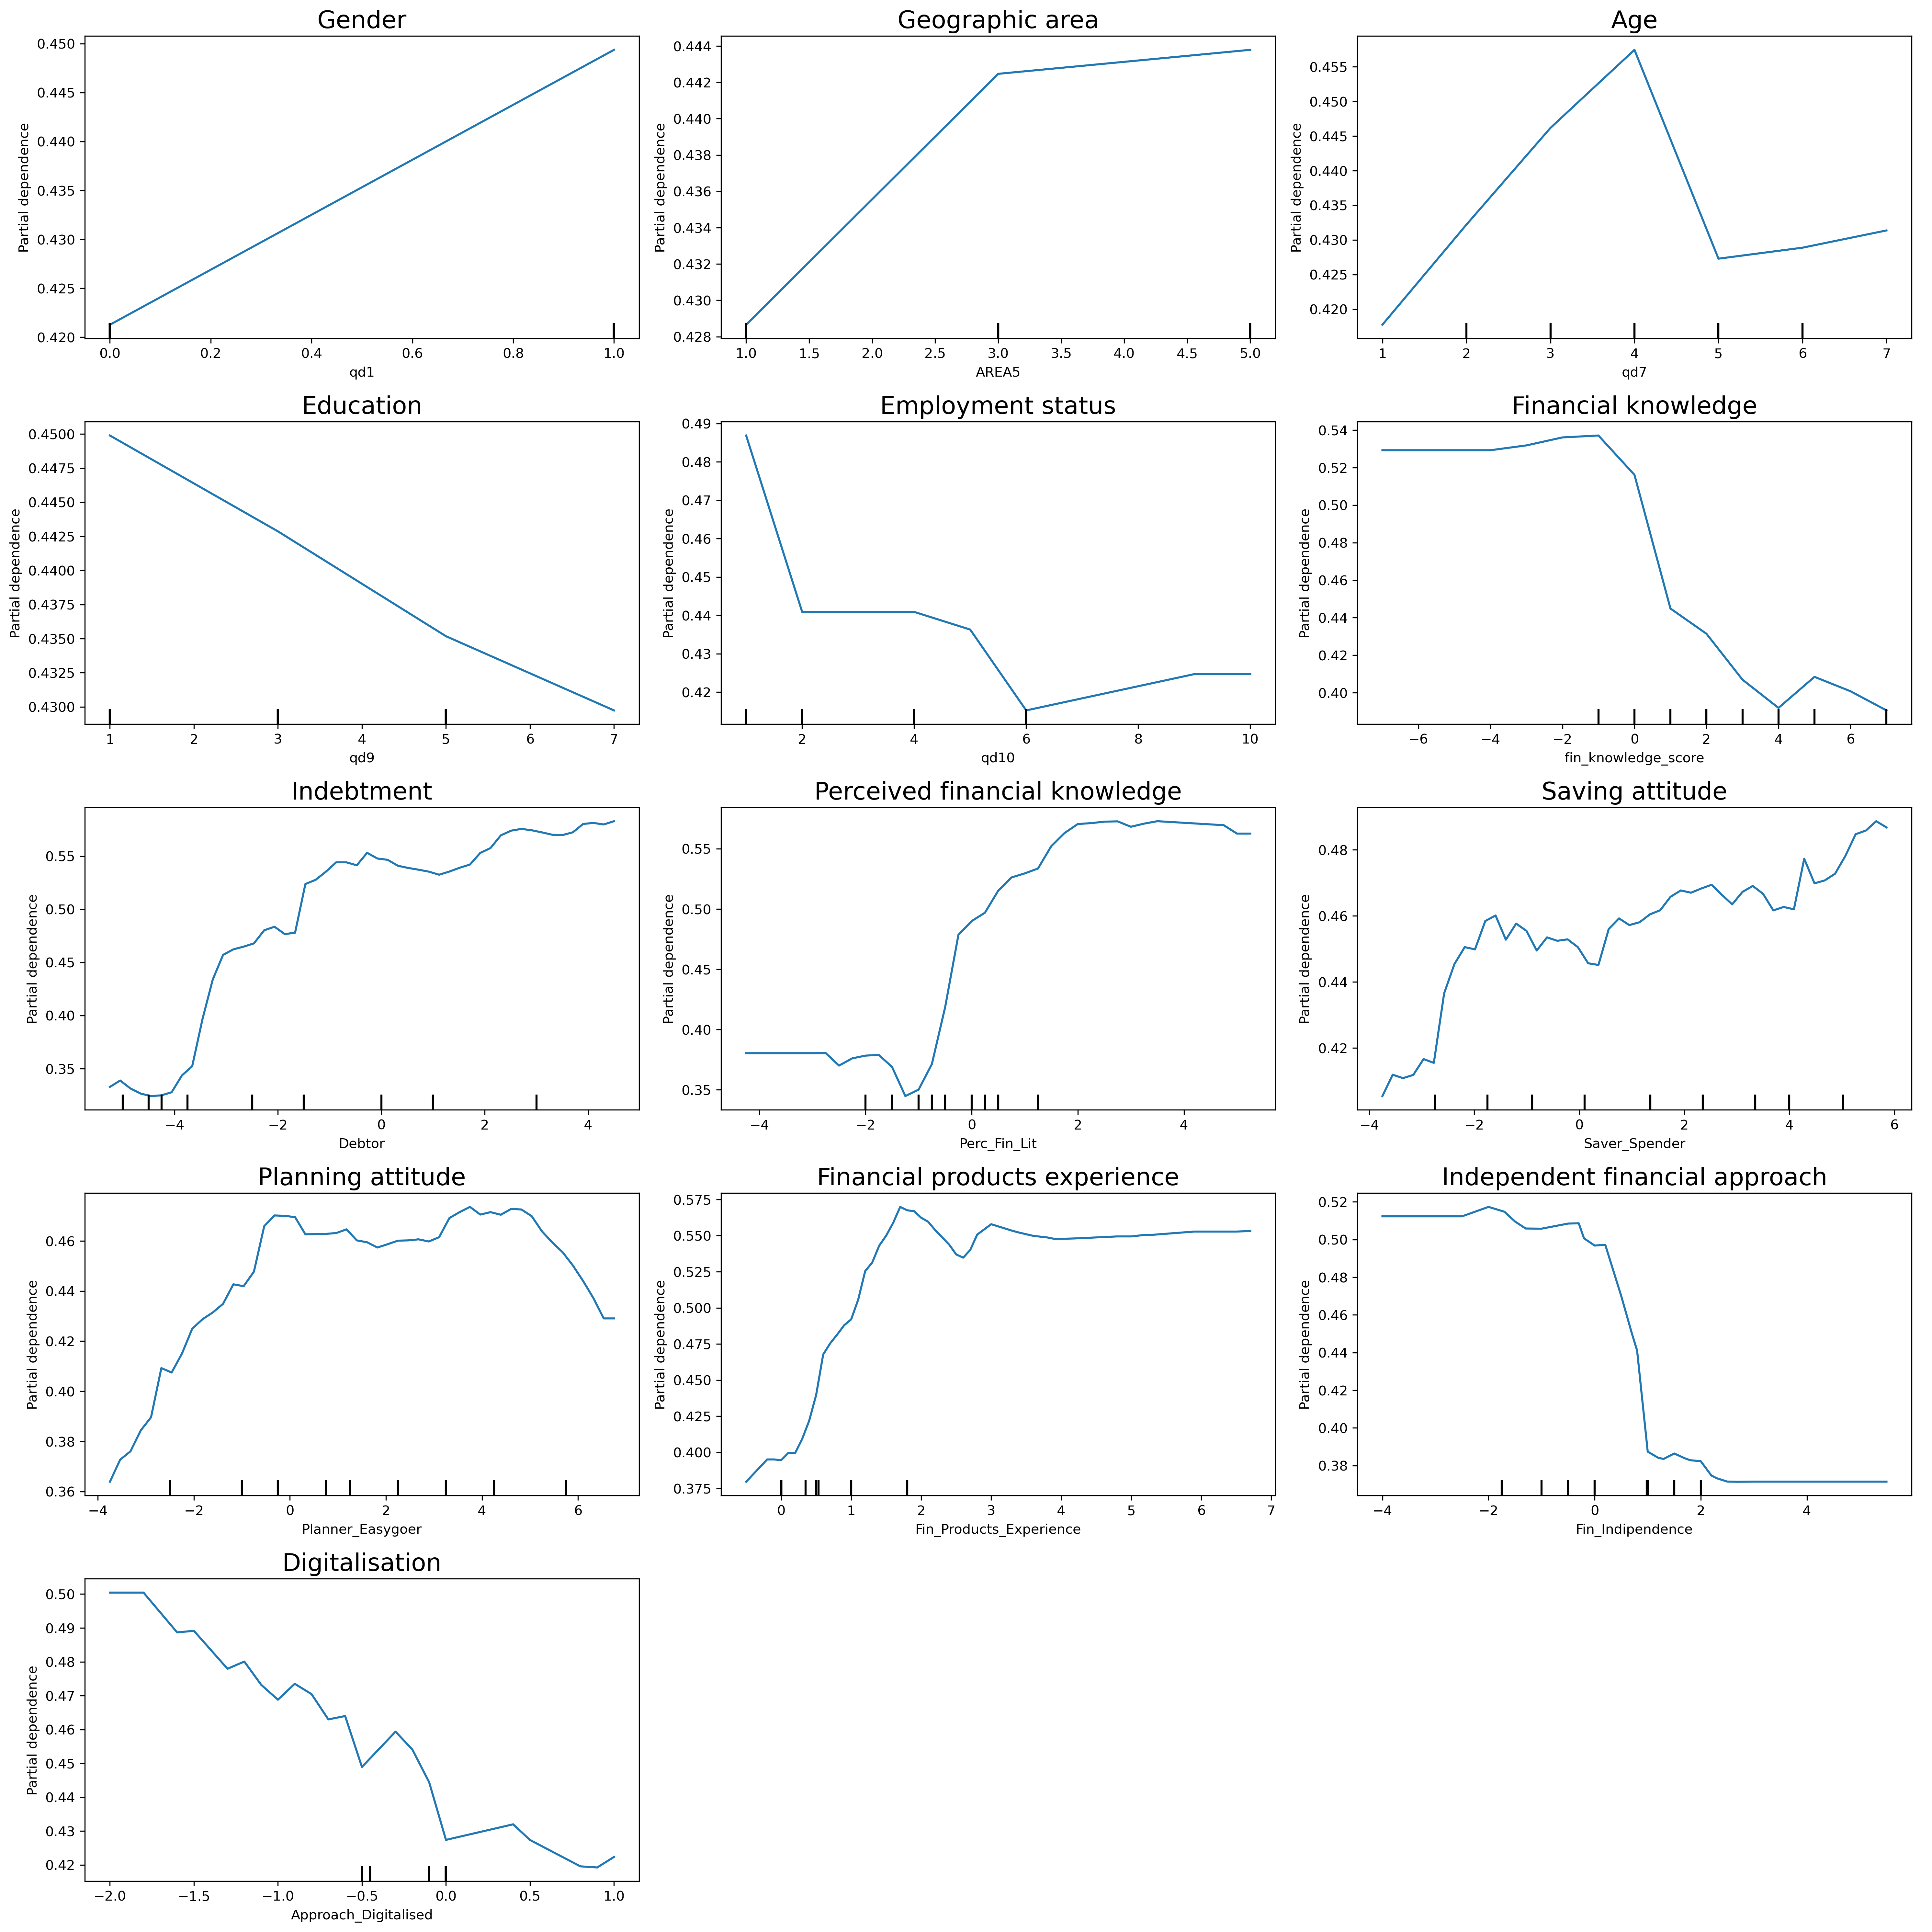
\includegraphics[height=16.5cm]{PartialDependences.png}
	%\includegraphics[width=7cm]{imm/grafico_potenza.png}
        %\includegraphics[width=7cm]{imm/log_potenza.png}
	%\captionsetup{format=hang}
 \caption{Feature partial dependencies with target variable}
 \label{partialdep}
\end{figure}

What can be seen here that is peculiar is how quickly the chances of being fraud victims rise with \textit{``Perceived financial knowledge"} and \textit{``Indebtment"}, and also with \textit{``Financial products experience"}. A surprise to be sure is instead the relationship that seem to arise between being a fraud victim and \textit{``Saving attitude"}: it looks like often times those who are defrauded also display a tendency on saving money and not spending it. This is probably due to the fact that it might be the case that those who are not interested in actively saving actually can't get hooked in financial frauds under the promise of a quick buck or more returns on investments. 

From our research question point of view, it's plots like the one for \textit{``Financial knowledge"} that show us how to combat fragility from a financial security standpoint in our society: by enhancing the financial knowledge of citizens. As soon as it reaches a basic level there is in fact a big drop in the dependence. 

\subsection{Units Out of Sample}
We can now try and take a look at different profiles which are clearly out of sample, but instructive because they might be examples of stereotypical people we meet or we can see ourselves into. 
\begin{table}[H]
  \begin{center}
  
    \resizebox{\columnwidth}{!}{\begin{tabular}{|l|c|c|c|c|c|c|}
    \hline
    \textbf{Features} & \textbf{Profile 1} & \textbf{Profile 2} & \textbf{Profile 3} & \textbf{Profile 4} & \textbf{Profile 5} & \textbf{Profile 6}\\
    \hline
    Gender & 1 & 0 & 1 & 0 & 1 & 0 \\ 
    Geographic area & 1 & 1 & 5 & 3 & 1 & 3 \\ 
    Age & 4 & 1 & 3 & 7 & 5 & 2\\
    Education & 1 & 1 & 5 & 7 & 3 & 1 \\
    Employment status & 2 & 9 & 5 & 6 & 1 & 2 \\
    Financial knowledge & -4 & -5 & -6 & -4 & -7 & 7 \\
    Indebtment & -4 & -5 & 3 & -5 & 8 & -1 \\
    Perceived financial knowledge & 1 & -2 & 5 & -4 & 6 & 6 \\
    Saving attitude & 11 & -4 & -5 & 12 & 2 & 7 \\
    Planning attitude & 7 & 4 & -4 & -6 & 0 & 8 \\
    Financial products experience & 5 & 1 & 1 & 6 & 3 & 8 \\
    Independent financial approach & 5 & -5 & 3 & 6 & 4 & 7 \\
    Digitalisation & -2 & 1 & -1 & -3 & 0 & 1 \\
    \hline
    \end{tabular}}
    
  \end{center}
 
  \caption{Six different profile creations}
  %\label{tab:prova1}
\end{table}

\begin{itemize}
    \item \textbf{Profile 1}: male adult aged 45-54 from Northern Italy, in full-time employment and with a university degree. Despite lacking financial expertise, he considers himself to possess a considerable amount of knowledge in this area and relies on his own understanding. He has a medium to high level of wealth, enabling him to have savings and no debts. He is reluctant to embrace technology
    \item \textbf{Profile 2}: female aged 18-25, from Northern Italy. She is a student with a bachelor's degree and is aware that her financial knowledge and experience with financial products are limited. Consequently, she seeks guidance from experts in these fields. Due to her lack of income, her financial resources are constrained, making it challenging for her to save and set ambitious long-term financial goals. However, she demonstrates a high level of digital proficiency
    \item \textbf{Profile 3}: male adult aged 35-44 from Southern Italy, seeking employment and possessing a primary school diploma. He considers himself to be knowledgeable about finance and therefore relies on his own expertise, however, evidence suggests otherwise. Lacking a stable income, he has limited financial resources, resulting in a lack of savings and an accumulation of debt that impedes his ability to plan for a secure future. Additionally, he exhibits a lack of confidence in technology
    \item \textbf{Profile 4}: elderly female, aged 75 and over, from central Italy, who has been retired for a number of years. She has some primary school certificate and, given her age, is aware that she lacks confidence in financial matters. However, she has gained some experience of financial products over the course of her life and, as a result, rarely seeks advice from family members or experts. As she is retired, she has no debts and saves money on small things, as she is unable to plan for the distant future. She has a negative attitude towards technology
    \item \textbf{Profile 5}: male adult aged 55-64 years old from Northern Italy. He is an entrepreneur with a high school diploma. He considers himself to be knowledgeable about finance and therefore relies on his own expertise, which is frequently demonstrated to be erroneous. His employment provides a satisfactory income, but he is unable to save due to the burden of multiple debts. He attempts to remain current with new technologies
    \item \textbf{Profile 6}: woman aged 25-34, hailing from central Italy. She is gainfully employed in a banking position and holds a university degree. She possesses exemplary financial acumen and experience, which she deems indispensable. She allocates a portion of her income to savings, and her financial obligations include a mortgage and regular installments, which are typical of individuals of her age. She is highly proficient in digital technologies 
\end{itemize}
The predicted probabilities for these out of sample units can be seen in figure [Fig.\ref{profile}]:
\begin{figure}[H]
  \centering
        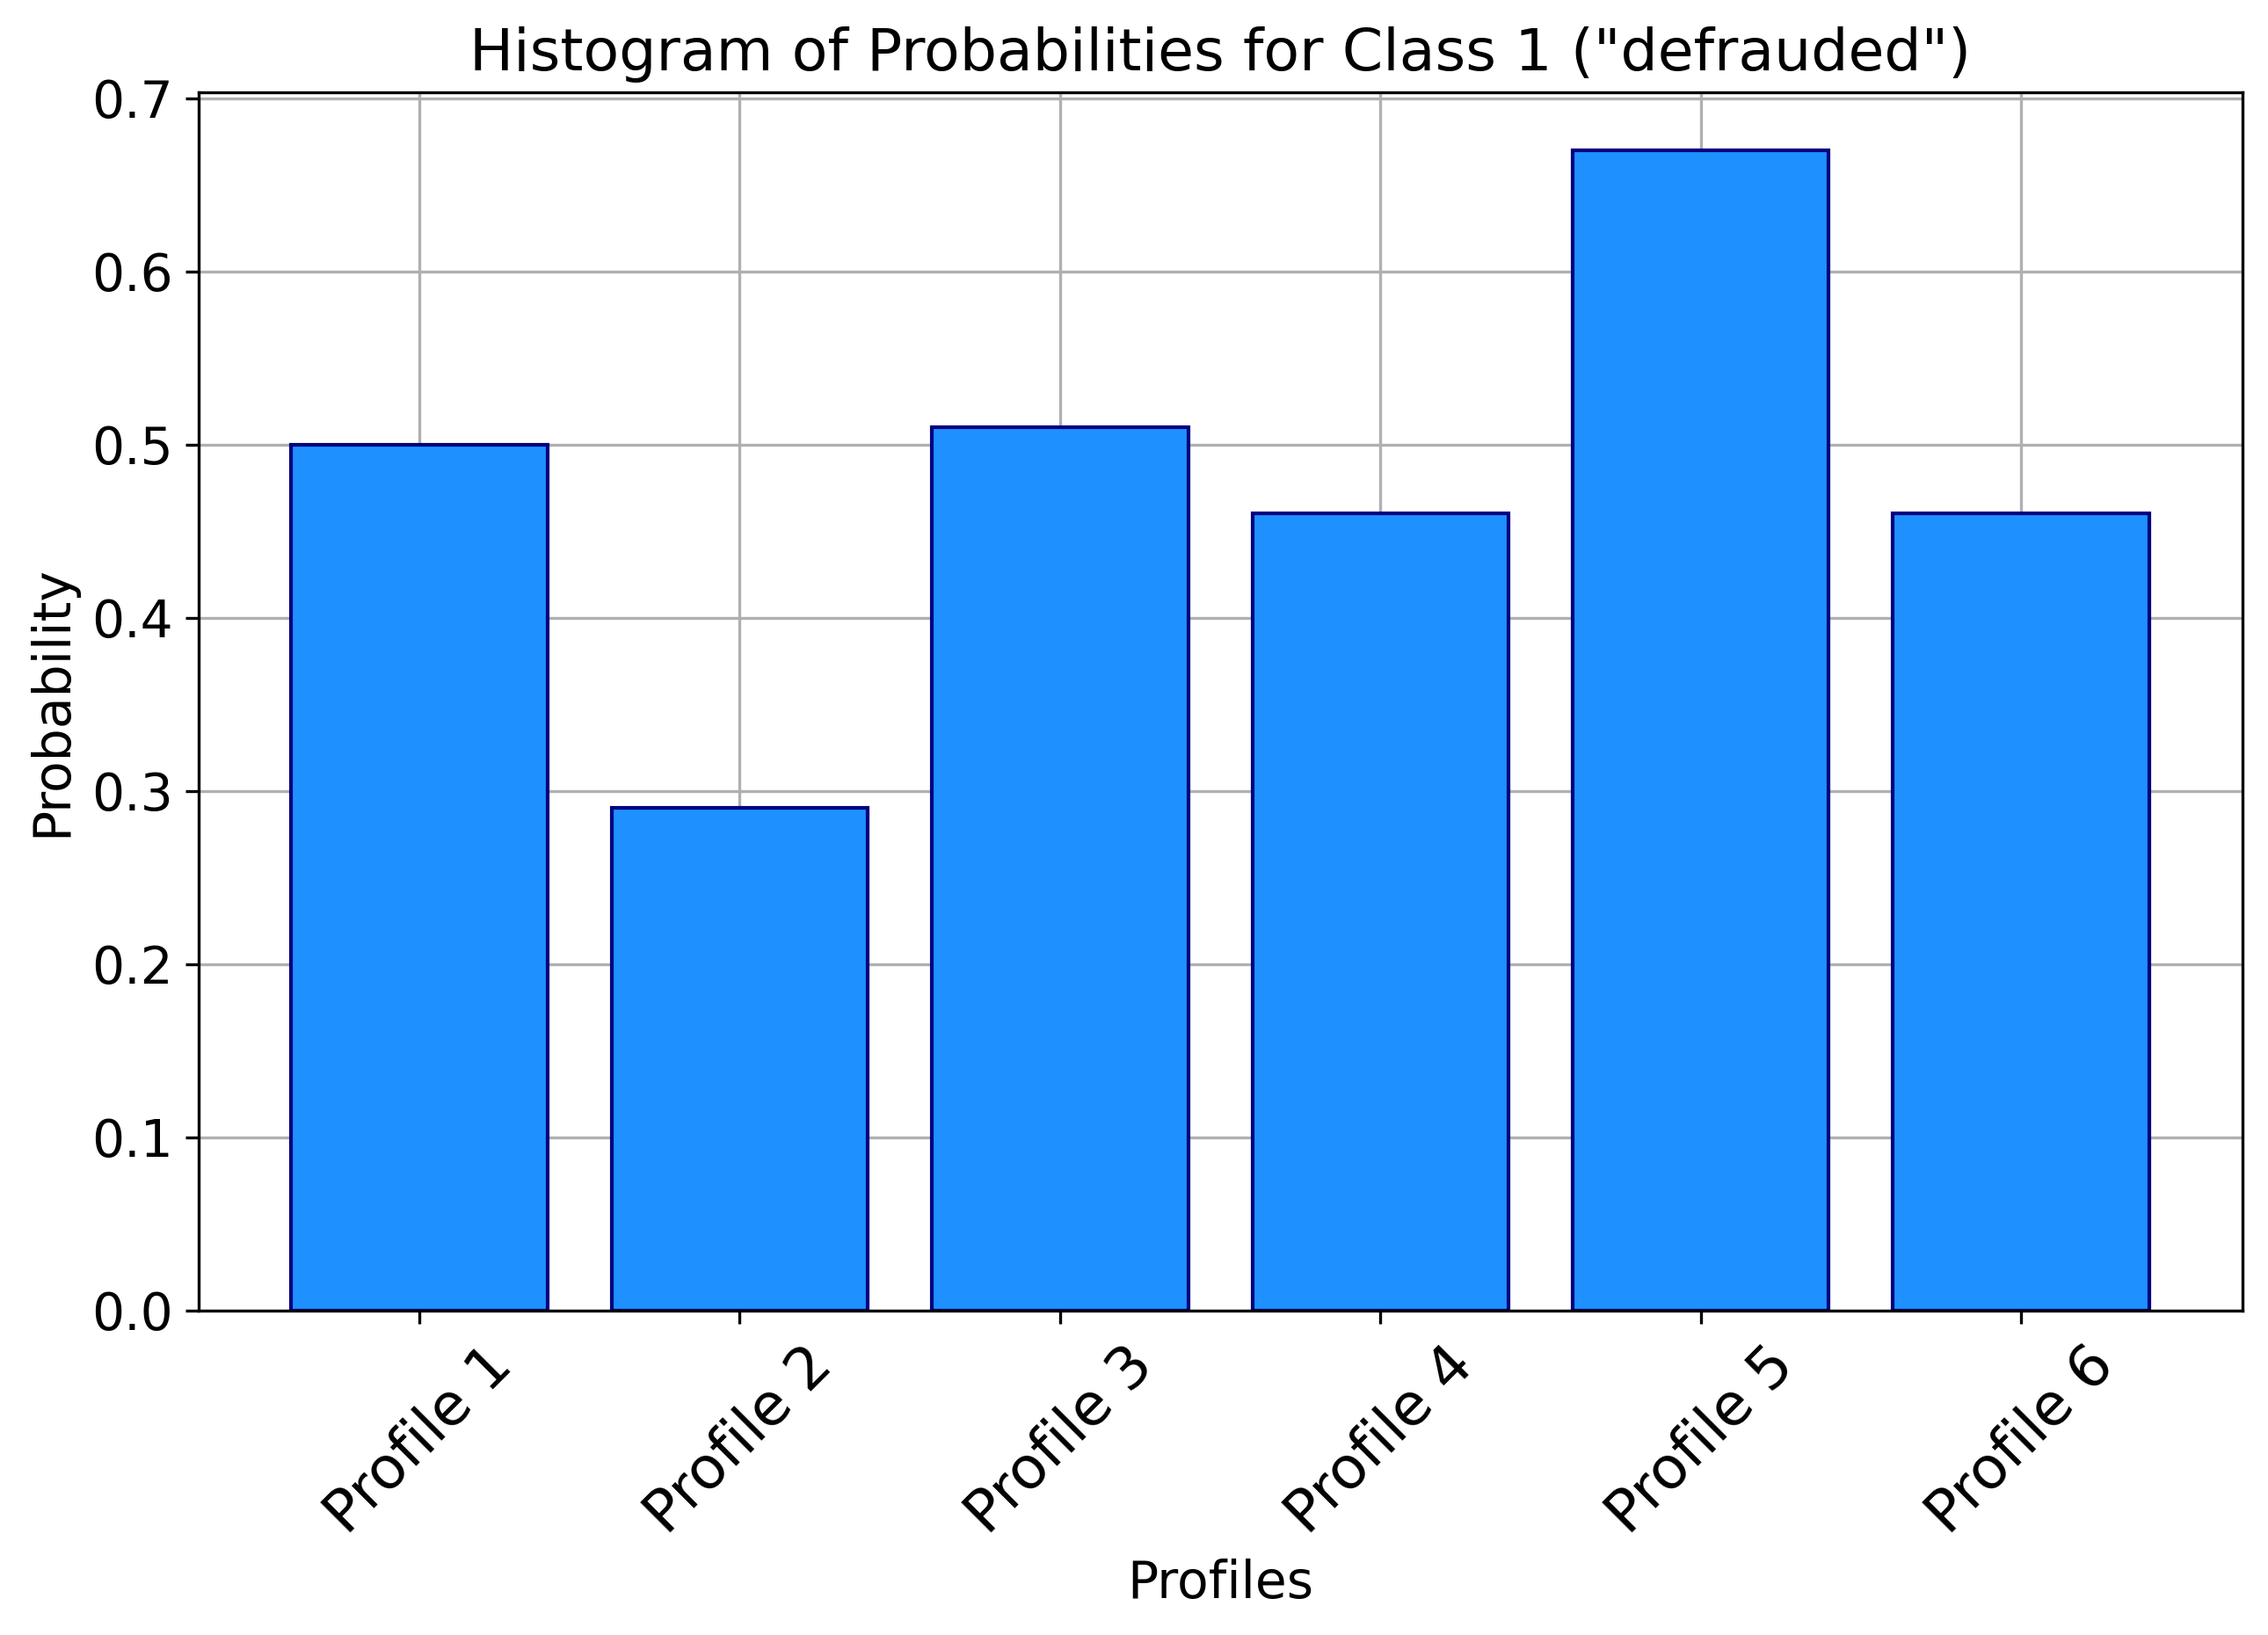
\includegraphics[width=12cm]{ProfileProbs.png}
	%\includegraphics[width=7cm]{imm/grafico_potenza.png}
        %\includegraphics[width=7cm]{imm/log_potenza.png}
	%\captionsetup{format=hang}
 \caption{Probabilities of six stereotypical profiles being defrauded}
 \label{profile}
\end{figure}

While most profiles are close to 0.5 and hence somewhat uncertain, we have two profiles that stand out quite a lot, one negatively (Profile 2) and one positively (Profile 5); we can see that the one that stood out negatively already had debt and perceived himself as knowledgeable about financial matters, while the one that stood out positively was generally debt averse and knew about its limitations around financial knowledge. Once again these two prove to be the most important factors. 

Another thing this plot shows is that profiles that we might think are not vulnerable, such as Profile 6, at last indeed seem quite vulnerable, and to some level being fraud victims is a transversal element of our society, sadly.

\section{Conclusion}
To conclude, does common knowledge identify fragile subjects? From our research the answer seems to be only partially yes, and for some other aspects no. For example, it is highlighted how fraud is a transversal aspect within the digital age; and moreover, not all common knowledge seems to be pointing out in the correct direction, such as in the case of partial dependencies for the saving attitude variable or in the case of Profile 6 of our out of sample profiles, in a manner that could be linked to the conjunction fallacy (also known as the ``Linda problem") \cite{Linda}. But still some aspects of common knowledge seem to emerge as correct from the inherent noise of the dataset: for example, the fact that being in debt makes someone much more vulnerable than others towards frauds, or also the matter of financial knowledge, which seems to be omnipresent and linked to many variables within the analysis. Especially regarding financial knowledge, it is interesting how it is usually pointed out as one of the first defense barriers against financial frauds, but it is peculiar how it is so not because of the information that it conveys to the one who possesses it but rather because it can disprove one's fallacies around the financial world, both in them being too sure of themselves and their behaviour and attitudes towards savings, debt, financial products and expectations of returns. 

At last, this research highlights once again another important albeit reiterated aspect: that fragile subjects are uniformly distributed across socio-demographic classes, meaning there is no particular correlation that is significant for sex, age, education or even digitalisation. 

This all means that any act that wants to reduce the vulnerability of the Italian population towards financial frauds has to act across many socio-demographic classes, with a particular accent on attitudes but also financial knowledge and also has to try and build measures and protective barriers around already financially stressed individuals. As always in a sense, complex problems cannot be reduced to simple and quick solutions but have to be thoroughly analyzed and require custom made solutions.

\section{Improvements}
Further improvements to this type of research are plenty, as an example we have:
\begin{itemize}
    \item the more data available the better: given other datasets with about the same imbalance (or a better one), being able to aggregate their data in the engineered features would mean being able to access new data points which can highlight new relationships; this presents many challenges that include, but are not limited to, the choice of how to reduce features to engineered ones; the ability to recreate effectively the target variable; the problem of noise in each dataset
    \item other approaches: approaches that might trade some interpretability for more complex models might work better in predicting if a person is more fragile and could ultimately lead to other insights; an example of such an approach could be clustering, or more complex ML models
    \item a different choice of data aggregation: from varying weights to considering different and less linear transformations to even changing the interaction between terms of the combinations, a different choice of data aggregation could lead to different insights; there would still be some systematic problems such as noise in the dataset because of inconsistencies but some problems could be resolved this way
    \item a more practical approach: rebuilding of the original dataset with new participants, maybe found through the internet or means where more anonymity is present, could bring about more data, or data that is best suited for the research question, or could even lead to create some tools that anyone can use to assess its fragility in the space of financial frauds
\end{itemize}


\newpage
\section{Appendices}
%\appendix
%\appendixpage

\subsection{Questionnaire used }\label{sec:appendix}

The \href{https://www.bancaditalia.it/statistiche/tematiche/indagini-famiglie-imprese/alfabetizzazione/Data-description.pdf?language_id=1}{questionnaire} consists of the following questions which correspond to columns of the analysed dataset:

\begin{itemize}
    \item \textit{\textbf{ID}}: Individual identifier
    \item \textit{\textbf{SM}}: Model of interview (0 - Tablet; 1 - CAPI)
    \item \textit{\textbf{PESOFITC}}: Sample weights
    \item \textit{\textbf{qd1}}: Gender (0 - Female; 1 - Male)
    \item \textit{\textbf{AREA5}}: Geographical area (1 - North-West; 2 - North-East; 3 - Centre; 4 - South; 5 - Islands)
    \item \textit{\textbf{qd5b}}: Number of household members (1 - One; 2 - Two; 3 -  Three; 4 - Four; 5 - Five; 6 - Six or more)
    \item \textit{\textbf{qd7}}: Age 
    \item \textit{\textbf{qd9}}: Educational qualification (1 - University-level education; 3 - Complete secondary school; 4 - Some secondary school; 5 - Complete primary school; 6 - Some primary school; 7 - No formal education)
    \item \textit{\textbf{qd10}}: Employment status (1 - Self-employed; 2 - In paid employment; 4 - Looking after the home; 5 - Looking for work; 6 - Retired; 9 - Student; 10 - Other)
    \item \textit{\textbf{qd12}}: Country of birth (1 - Italy; 0 - Abroad)
    \item \textit{\textbf{qf1}}: Who is responsible for making day-to-day decisions about money in your household? (1 - You make these decisions by yourself; 2 - You make these decisions with other household members; 3 - Other household members, not you; -99 - No answer)
    \item \textit{\textbf{qf2}}: The next question is about the household budget. A household budget is used to plan what share of your household income will be used for spending or saving. Does your household have a budget to plan in advance which share of income will be used for spending and which share will be saved for the next years? (1 - Yes; 0 - No; -99 - No answer) 
    \item \textit{\textbf{qf3\_1 - qf3\_99}}: In the past 12 months have you been personally saving money in any of the following ways, whether or not you still have the money? Please do not include pension savings.
    \begin{itemize}
        \item \textit{\textbf{qf3\_1}}: Saving cash at home or in your wallet 
        \item \textit{\textbf{qf3\_3}}: Paying money into a savings account
        \item \textit{\textbf{qf3\_4}}: Giving money to family to save on your behalf
        \item \textit{\textbf{qf3\_6}}: Buying financial investment products, other than pension funds (e.g. bonds, shares, mutual funds)
        \item \textit{\textbf{qf3\_7}}: Or in some other way (including remittances, buying livestock, gold or property)
        \item \textit{\textbf{qf3\_8}}: Has not been actively saving
        \item \textit{\textbf{qf3\_99}}: No answer 
    \end{itemize}
    \item \textit{\textbf{qf4}}: And if you, personally, faced a major expense today, equivalent to your own monthly income, would you be able to pay it without borrowing the money or asking family or friends to help? (1 - Yes; 0 - No; -97 - Don't know; -98 - I don't have a personal income; -99 - No answer)
    \item \textit{\textbf{qf8}}: Overall, how confident are you that you have done a good job of making financial plans for your retirement? 
    (1 - Very confident; 2 - Confident; 3 - Somehow confident; 4 - Not very confident; 5 - Not at all confident; 6 - I’m not planning for retirement; -97 - Don't know; -99 - No answer)
    
    \item \textit{\textbf{qf9\_1 - qf9\_99}}: And how will you - or do you - fund your retirement? 
    \begin{itemize}
        \item \textit{\textbf{qf9\_1}}: From drawing a government pension/old-age benefit 
        \item \textit{\textbf{qf9\_2}}: From an occupational or workplace pension plan 
        \item \textit{\textbf{qf9\_3}}: From a private pension plan
        \item \textit{\textbf{qf9\_4}}: From selling your financial assets (such as stocks, bonds or mutual funds)
        \item \textit{\textbf{qf9\_5}}: From selling your non-financial assets (such as a car, property, art, jewels, antiques)
        \item \textit{\textbf{qf9\_6}}: From income generated by your financial or non-financial assets
        \item \textit{\textbf{qf9\_7}}: By relying on a spouse or partner to support you
        \item \textit{\textbf{qf9\_8}}: By relying on your children or other family members to support you
        \item \textit{\textbf{qf9\_9}}: Survivor’s pension
        \item \textit{\textbf{qf9\_10}}: Other
        \item \textit{\textbf{qf9\_99}}: No answer
    \end{itemize}
    
    \item \textit{\textbf{qprod1c\_1 - qprod1c\_99}}: In the last two years, which of the following types of financial products have you bought, whether or not you still hold them? 
    \begin{itemize}
        \item \textit{\textbf{qprod1c\_1}}: A pension or retirement product
        \item \textit{\textbf{qprod1c\_2}}: An investment account such as a unit trust
        \item \textit{\textbf{qprod1c\_3}}: A mortgage or a bank loan secured on a property
        \item \textit{\textbf{qprod1c\_5}}: An unsecured bank loan or a salary/pension-backed loan
        \item \textit{\textbf{qprod1c\_6}}: A credit card
        \item \textit{\textbf{qprod1c\_7}}: A current/checking account
        \item \textit{\textbf{qprod1c\_8}}: A savings account
        \item \textit{\textbf{qprod1c\_10}}: Insurance
        \item \textit{\textbf{qprod1c\_11}}: Stocks and shares
        \item \textit{\textbf{qprod1c\_12}}: Bonds
        \item \textit{\textbf{qprod1c\_14}}: A prepaid debit card/payment card
        \item \textit{\textbf{qprod1c\_99}}: No answer
    \end{itemize}
    
    \item \textit{\textbf{qprod1\_d}}: Which of these did you choose most recently? (If at least one product was selected go to \textit{prod1\_d}, otherwise go to \textit{qf10})

    \item \textit{\textbf{qprod2}}: Which of the following statements best describes how you made your choice? 
    (1 - I considered several options from different companies before making my decision; 2 - I considered the various options from one company; 3 - I didn’t consider any other options at all; 4 - I looked around but there were no other options to consider; -99 - No answer)

    \item \textit{\textbf{qprod3\_1 - qprod3\_99}}: Which sources of information do you feel most influenced your decision?
    \begin{itemize}
        \item \textit{\textbf{qprod3\_1}}: Unsolicited information sent through the post
        \item \textit{\textbf{qprod3\_2}}: Information picked up in a branch
        \item \textit{\textbf{qprod3\_3}}: Product specific information found on the internet
        \item \textit{\textbf{qprod3\_4}}: Information from sales staff of the firm providing the products
        \item \textit{\textbf{qprod3\_5}}: Best-buy tables in financial pages of newspapers/magazines
        \item \textit{\textbf{qprod3\_6}}: Best-buy information found on the internet
        \item \textit{\textbf{qprod3\_7}}: Specialist magazines/publications
        \item \textit{\textbf{qprod3\_8}}: Recommendation from independent financial adviser or broker
        \item \textit{\textbf{qprod3\_9}}: Advice of friends/relatives (not working in the financial services industry)
        \item \textit{\textbf{qprod3\_10}}: Advice of friends/relatives (who work in the financial services industry)
        \item \textit{\textbf{qprod3\_11}}: Employer’s advice
        \item \textit{\textbf{qprod3\_12}}: Newspaper articles
        \item \textit{\textbf{qprod3\_13}}: Television or radio programs
        \item \textit{\textbf{qprod3\_14}}: Newspaper adverts
        \item \textit{\textbf{qprod3\_15}}: Television adverts
        \item \textit{\textbf{qprod3\_16}}: Other advertising
        \item \textit{\textbf{qprod3\_17}}: My own previous experience
        \item \textit{\textbf{qprod3\_18}}: Other source
        \item \textit{\textbf{qprod3\_99}}: No answer
    \end{itemize}

    \item \textit{\textbf{qf10\_1 - qf10\_12}}: I am now going to read out some statements. I would like to know how much you agree or disagree that each of the statements applies to you, personally. Please use a scale of 1 to 5, where 1 tells me that you completely agree that the statement describes you, while 5 shows that you completely disagree (1 = Totally agrees, 5 = Totally disagrees, -97 = Don’t know, -99 = No answer) 
    \begin{itemize}
        \item \textit{\textbf{qf10\_1}}: Before I buy something I carefully consider whether I can afford it
        \item \textit{\textbf{qf10\_2}}: I tend to live for today and let tomorrow take care of itself
        \item \textit{\textbf{qf10\_3}}: I find it more satisfying to spend money than to save it for the long term
        \item \textit{\textbf{qf10\_4}}: I pay my bills on time
        \item \textit{\textbf{qf10\_5}}: I am prepared to risk some of my own money when saving or making an investment
        \item \textit{\textbf{qf10\_6}}: I keep a close personal watch on my financial affairs
        \item \textit{\textbf{qf10\_7}}: I set long-term financial goals and strive to achieve them
        \item \textit{\textbf{qf10\_8}}: Money is there to be spent
        \item \textit{\textbf{qf10\_9}}: My financial situation limits my ability to do the things that are important to me
        \item \textit{\textbf{qf10\_10}}: I tend to worry about paying my normal living expenses
        \item \textit{\textbf{qf10\_11}}: I have too much debt right now
        \item \textit{\textbf{qf10\_12}}: I am satisfied with my present financial situation
    \end{itemize}
    
    \item \textit{\textbf{qprod4\_1 - qprod4\_3}}: Thinking about financial products and services in general, in the last 2 years, have you experienced any of the following issues? (1 = True, 0 = False, -95 = I don't understand, -97 = I don’t know, -99 = I prefer not to answer)
    \begin{itemize}
        \item \textit{\textbf{qprod4\_1}}: You accepted advice to invest in a financial product that you later found to be worthless
        \item \textit{\textbf{qprod4\_2}}: You accidentally provided financial information in response to an email or phone call that you later found out was not genuine
        \item \textit{\textbf{qprod4\_3}}: You discovered that someone had used your cards or personal information to pay for goods without your authorization
    \end{itemize}

    \item \textit{\textbf{qk1}}: And now we talk about financial literacy. Could you tell me how you would rate your overall knowledge about financial matters? 
    (1 - Well above average; 2 - Above average; 3 - Average; 4 - Below average; 5 - Well below average; -97 - Don't know; -99 - No answer)

    \item \textit{\textbf{qf11}}: Sometimes people find that their income does not quite cover their living costs. In the last 12 months, has this happened to you, personally? 
    (1 - Yes; 0 - No; -99 - No answer)

    \item \textit{\textbf{qf12\_1\_a - qf12\_99}}: What did you do to make ends meet the last time this happened?
    \begin{itemize}
        \item \textit{\textbf{qf12\_1\_a}}: Draw money out of savings
        \item \textit{\textbf{qf12\_1\_b}}: Cut back on spending, spend less, do without
        \item \textit{\textbf{qf12\_1\_c}}: Sell something that you own
        \item \textit{\textbf{qf12\_2\_d}}: Work overtime, earn extra money
        \item \textit{\textbf{qf12\_3\_e}}: Borrow from family or friends
        \item \textit{\textbf{qf12\_3\_f}}: Borrow from employer/salary advance
        \item \textit{\textbf{qf12\_3\_g}}: Pawn something that you own
        \item \textit{\textbf{qf12\_4\_k}}: Use authorized, arranged overdraft or line of credit
        \item \textit{\textbf{qf12\_4\_l}}: Use credit card for a cash advance or to pay bills/buy food
        \item \textit{\textbf{qf12\_5\_m}}: Take out a personal loan from a financial service provider (including bank, credit union or microfinance)
        \item \textit{\textbf{qf12\_5\_o}}: Take out a loan from an informal provider/moneylender
        \item \textit{\textbf{qf12\_6\_p}}: Use unauthorized overdraft
        \item \textit{\textbf{qf12\_6\_q}}: Pay my bills late; miss payments
        \item \textit{\textbf{qf12\_7\_r}}: Other
        \item \textit{\textbf{qf12\_97}}: Don't know
        \item \textit{\textbf{qf12\_99}}: No answer
    \end{itemize}

    \item \textit{\textbf{qf13}}: If you lost your main source of household income, how long could your household continue to cover living expenses, without borrowing any money? 
    (1 - Less than a week; 2 - At least a week, but not one month; 3 - At least one month, but not three months; 4 - At least three months, but not six months; 5 - More than six months; -97 - Don't know; -99 - No answer)

    \item \textit{\textbf{qk3}}: Assume that you receive a gift of \euro{}1,000. Imagine that you have to wait for one year to get it and inflation stays at 1\%. In one year’s time will you be able to buy:
    (1 - More than you could today; 2 - The same amount; 3 - Less than you could buy today; -97 - Don't know; -99 - No answer)

    \item \textit{\textbf{qk4}}: You lend \euro{}25 to a friend one evening and he gives you \euro{}25 back the next day. How much interest has he paid on this loan? 
    (Numeric answer; -97 - Don't know; -99 - No answer)

    \item \textit{\textbf{qk5}}: Suppose you put \euro{}100 into a \textless no fee, tax free\textgreater savings account with a guaranteed interest rate of 2\% per year. How much would be in the account at the end of the first year, once the interest payment is made? 
    (Numeric answer; -97 - Don't know; -99 - No answer)

    \item \textit{\textbf{qk6}}: And how much would be in the account at the end of five years [remembering there are no fees or tax deductions and you don’t make any further payments into this account and you don’t withdraw any money]? 
    (1 - More than \euro{}110; 2 - \euro{}110; 3 - Less than \euro{}110; 4 - It is impossible to tell from the information given; -97 - Don't know; -99 - No answer)

    \item \textit{\textbf{qk7\_1 - qk7\_3}}: I would like to know whether you think the following statements are true or false: (1 - True; 0 - False; -97 - Don't know; -99 - No answer)
    \begin{itemize}
        \item \textit{\textbf{qk7\_1}}: An investment with a high return is likely to be high risk. 
        \item \textit{\textbf{qk7\_2}}: High inflation means that the cost of living is increasing rapidly
        \item \textit{\textbf{qk7\_3}}: It is usually possible to reduce the risk of investing in the stock market by buying a wide range of stocks and shares
    \end{itemize}
\end{itemize}

\newpage
\subsection{Feature Engineering matrix and rules}\label{sec:coeffweights}

\begin{table}[H]
  \begin{center}
  
    \resizebox{\columnwidth}{!}{\begin{tabular}{|l|c|c|c|c|c|c|c|c|}
    \hline
    \textbf{} & \makecell{\textbf{Financial} \\ \textbf{knowledge}} & \textbf{Indebtment} & \makecell{\textbf{Perceived} \\ \textbf{fin. knowledge}} & \makecell{\textbf{Saving} \\ \textbf{attitude}} & \makecell{\textbf{Planning} \\ \textbf{attitude}} & \makecell{\textbf{Financial products} \\ \textbf{experience}} & \makecell{\textbf{Independent} \\ \textbf{fin. approach}} & \textbf{Digitalisation}\\
    \hline
    \textit{\textbf{qf1}} & 0 & 0 & 0 & 0 & 1.0 & 0 & 1.0 & 0 \\
    \textit{\textbf{qf2}} & 0 & 0 & 0 & 0 & 0.5 & 0 & 0 & 0 \\
    \textit{\textbf{qf3\_1}} & 0 & 0 & 0 & 2.0 & 0 & 0.3 & 0.5 & -0.5 \\
    \textit{\textbf{qf3\_3}} & 0 & 0 & 0 & 2.0 & 0 & 0.5 & 0 & 0 \\
    \textit{\textbf{qf3\_4}} & 0 & 0 & 0 & 2.0 & 0 & -0.5 & -1.0 & -0.5 \\
    \textit{\textbf{qf3\_6}} & 0 & 0 & 0 & 1.0 & 0 & 1.5 & 0 & 0 \\
    \textit{\textbf{qf3\_7}} & 0 & 0 & 0 & 1.0 & 0 & 1.0 & 0 & 0 \\
    \textit{\textbf{qf3\_8}} & 0 & 0 & 0 & -2.0 & 0 & 0 & 0 & 0 \\
    \textit{\textbf{qf4}} & 0 & 0 & 0 & 0.5 & 1.0 & 0 & 1.0 & 0 \\
    \textit{\textbf{qf8}} & 0 & 0 & 1.0 & 0 & 0 & 0 & 0 & 0 \\
    \textit{\textbf{qf9\_1\_9}} & 0 & 0 & 0 & 0 & 1.0 & 0 & 0 & 0 \\
    \textit{\textbf{qf9\_2\_3}} & 0 & 0 & 0 & 0 & 1.0 & 0 & 0 & 0 \\
    \textit{\textbf{qf9\_4}} & 0 & 0 & 0 & 0 & 1.0 & 1.0 & 0.8 & 0 \\
    \textit{\textbf{qf9\_5}} & 0 & 0 & 0 & 0 & 1.0 & 0 & 1.0 & 0 \\
    \textit{\textbf{qf9\_6}} & 0 & 0 & 0 & 0 & 1.0 & 0 & 1.0 & 0 \\
    \textit{\textbf{qf9\_7\_8}} & 0 & 0 & 0 & 0 & 0 & 0 & -1.0 & 0 \\
    \textit{\textbf{qprod1c\_1}} & 0 & 0 & 0 & 0 & 0 & 0.6 & 0 & 0 \\
    \textit{\textbf{qprod1c\_2}} & 0 & 0 & 0 & 0 & 0 & 0.9 & 0 & 0 \\
    \textit{\textbf{qprod1c\_3}} & 0 & 1.0 & 0 & 0 & 0 & 0.4 & 0 & 0 \\
    \textit{\textbf{qprod1c\_5}} & 0 & 0.5 & 0 & 0 & 0 & 0 & 0 & 0 \\
    \textit{\textbf{qprod1c\_6}} & 0 & 0 & 0 & 0 & 0 & 1.0 & 0 & 0 \\
    \textit{\textbf{qprod1c\_7}} & 0 & 0 & 0 & 1.0 & 0 & 0.3 & 0 & 0 \\
    \textit{\textbf{qprod1c\_8}} & 0 & 0 & 0 & 1.0 & 0 & 0.6 & 0 & 0 \\
    \textit{\textbf{qprod1c\_10}} & 0 & 0 & 0 & 0 & 0 & 0.1 & 0 & 0 \\
    \textit{\textbf{qprod1c\_11}} & 0 & 0 & 0 & 0 & 0 & 1.0 & 0 & 0 \\
    \textit{\textbf{qprod1c\_12}} & 0 & 0 & 0 & 0 & 0 & 1.0 & 0 & 0 \\
    \textit{\textbf{qprod1c\_14}} & 0 & 0 & 0 & 0 & 0 & 0.4 & 0 & 0 \\
    \textit{\textbf{qprod2}} & 0 & 0 & 1.0 & 0 & 0 & 0 & 0 & 0 \\
    \textit{\textbf{qprod3\_1\_16}} & 0 & 0 & 0 & 0 & 0 & 0 & 0 & -0.3 \\
    \textit{\textbf{qprod3\_2}} & 0 & 0 & 0 & 0 & 0 & 0 & 0 & -0.3 \\
    \textit{\textbf{qprod3\_3\_6}} & 0 & 0 & 0 & 0 & 0 & 0 & 0 & 1.0 \\
    \textit{\textbf{qprod3\_4}} & 0 & 0 & 0 & 0 & 0 & 0 & -0.5 & -0.2 \\
    \textit{\textbf{qprod3\_5\_7\_12\_14}} & 0 & 0 & 0 & 0 & 0 & 0 & 0 & -1.0 \\
    \textit{\textbf{qprod3\_8}} & 0 & 0 & 0 & 0 & 0 & 0 & -1.0 & -0.1 \\
    \textit{\textbf{qprod3\_9}} & 0 & 0 & 0 & 0 & 0 & 0 & -1.0 & 0 \\
    \textit{\textbf{qprod3\_10}} & 0 & 0 & 0 & 0 & 0 & 0 & -1.0 & 0 \\
    \textit{\textbf{qprod3\_11}} & 0 & 0 & 0 & 0 & 0 & 0 & -0.5 & 0 \\
    \textit{\textbf{qprod3\_13\_15}} & 0 & 0 & 0 & 0 & 0 & 0 & 0 & -0.1 \\
    \textit{\textbf{qprod3\_17}} & 0 & 0 & 0.5 & 0 & 0 & 0 & 0.7 & 0 \\
    \textit{\textbf{qf10\_1}} & 0 & 0 & 0 & 0.5 & 0 & 0 & 0 & 0 \\
    \textit{\textbf{qf10\_2}} & 0 & 0 & 0 & 0 & -1.0 & 0 & 0 & 0 \\
    \textit{\textbf{qf10\_3}} & 0 & 0 & 0 & -0.5 & 0 & 0 & 0 & 0 \\
    \textit{\textbf{qf10\_4}} & 0 & -0.25 & 0 & 0 & 0 & 0 & 0 & 0 \\
    \textit{\textbf{qf10\_5}} & 0 & 0 & 0 & 0.5 & 1.0 & 0 & 0 & 0 \\
    \textit{\textbf{qf10\_6}} & 0 & 0 & 0.25 & 0 & 0.5 & 0 & 0 & 0 \\
    \textit{\textbf{qf10\_7}} & 0 & 0 & 0 & 0 & 1.0 & 0 & 0 & 0 \\
    \textit{\textbf{qf10\_8}} & 0 & 0 & 0 & -0.5 & 0 & 0 & 0 & 0 \\
    \textit{\textbf{qf10\_9}} & 0 & 0.25 & 0 & 0 & 0 & 0 & 0 & 0 \\
    \textit{\textbf{qf10\_10}} & 0 & 0.25 & 0 & 0 & 0 & 0 & 0 & 0 \\
    \textit{\textbf{qf10\_11}} & 0 & 2.0 & 0 & 0 & 0 & 0 & 0 & 0 \\
    \textit{\textbf{qf10\_12}} & 0 & 0 & 0.25 & 0 & 0 & 0 & 0 & 0 \\
    \textit{\textbf{qk1}} & 0 & 0 & 1.0 & 0 & 0 & 0 & 0 & 0 \\
    \textit{\textbf{qf11}} & 0 & 0 & 0 & -2.0 & 0 & 0 & 0 & 0 \\
    \textit{\textbf{qf12\_1\_a}} & 0 & 0 & 0 & 0.5 & 0 & 0 & 0 & 0 \\
    \textit{\textbf{qf12\_1\_b}} & 0 & 0 & 0 & 1.0 & 0 & 0 & 1.0 & 0 \\
    \textit{\textbf{qf12\_1c\_3g}} & 0 & 0 & 0 & 0 & 0 & 0 & 1.0 & 0 \\
    \textit{\textbf{qf12\_2d}} & 0 & 0 & 0 & 0 & 0 & 0 & 1.0 & 0 \\
    \textit{\textbf{qf12\_3e}} & 0 & 1.0 & 0 & 0 & 0 & 0 & -1.0 & 0 \\
    \textit{\textbf{qf12\_3f}} & 0 & 1.0 & 0 & 0 & 0 & 0 & -1.0 & 0 \\
    \textit{\textbf{qf12\_4k\_5m\_5o\_6p}} & 0 & 1.0 & 0 & 0 & 0 & 0 & -1.0 & 0 \\
    \textit{\textbf{qf12\_4l}} & 0 & 0 & 0 & 0 & 0 & 0 & 1.0 & 0 \\
    \textit{\textbf{qf12\_6q}} & 0 & 0.5 & 0 & 0 & 0 & 0 & 0 & 0 \\
    \textit{\textbf{qf13}} & 0 & 0 & 0 & 0.25 & 0.25 & 0 & 0 & 0 \\
    \textit{\textbf{qk3}} & $1/3$ & 0 & 0 & 0 & 0 & 0 & 0 & 0 \\
    \textit{\textbf{qk4}} & $1/3$ & 0 & 0 & 0 & 0 & 0 & 0 & 0 \\
    \textit{\textbf{qk5}} & $1/3$ & 0 & 0 & 0 & 0 & 0 & 0 & 0 \\
    \textit{\textbf{qk6}} & $1/3$ & 0 & 0 & 0 & 0 & 0 & 0 & 0 \\
    \textit{\textbf{qk7\_1}} & $1/3$ & 0 & 0 & 0 & 0 & 0 & 0 & 0 \\
    \textit{\textbf{qk7\_2}} & $1/3$ & 0 & 0 & 0 & 0 & 0 & 0 & 0 \\
    \textit{\textbf{qk7\_3}} & $1/3$ & 0 & 0 & 0 & 0 & 0 & 0 & 0 \\
    \hline
    \end{tabular}}
    
  \end{center}

  %\vspace{-0.5cm}
  %\caption{Six different profile creations}
  %\label{tab:prova1}
\end{table}
How to read and use the matrix: let A be a respondent and $\hat{S_A}$ its transformed score for all questions (rows) of the matrix above, M. 
Then, the vector of values of all new features V (present as matrix columns) can be computed as $V=\hat{S_A} * M$. Note that $\hat{S_A}$ is NOT exactly the vector of score $S_A$ for all question but has instead to follow certain rules for its transformation: 

\begin{itemize}
    \item score for question \textit{``qf8"} is changed as following $\hat{S_A}(qf8)=\Bar{X}-X_i$ where $\Bar{X}$ is the average of possible scores and $X_i$ is the score of the i-th row; the same applies to scores from \textit{``qf10\_i"} and \textit{``qprod3\_i"} 
    $\forall i$, \textit{``qk1"} and \textit{``qf1"}
    
    \item for \textit{``qf13"}, \textit{``qf2"}, \textit{``qf1"}, \textit{``qf4"}, \textit{``qf11"}, \textit{``qk1"}, \textit{``qf8"}, all \textit{``qf12\_i"}, all scores become zero when they are -99 or -97 or 6 (in the case of \textit{8})
    
    \item for \textit{``qf4"} if the score is 2 it becomes zero; moreover, if the score is used to compute values for the independent financial approach variable then if the score is zero it becomes -1

    \item for \textit{``qf11"} if the score is zero it becomes 0.5

    \item for all \textit{``qf9\_i"} features when included in the planning attitude variable the scores are summed and when positive becomes one, otherwise stays zero. The same applies for the features \textit{``qf12\_1\_b"}, \textit{``qf12\_1c\_3g"}, \textit{``qf12\_2\_d"} and \textit{``qf12\_4\_l"} when included in the independent financial approach variable; and in the same financial approach variable also this applies to features \textit{``qf12\_3\_f"}, \textit{``qf12\_3\_e"} and \textit{``qf12\_4k\_5m\_5o\_6p"}
\end{itemize}
So, to obtain the transformed $\hat{S_A}$, one applies all rules to the simple $S_A$ score.

\newpage
\printbibliography

\end{document}


